% Options for packages loaded elsewhere
% Options for packages loaded elsewhere
\PassOptionsToPackage{unicode}{hyperref}
\PassOptionsToPackage{hyphens}{url}
\PassOptionsToPackage{dvipsnames,svgnames,x11names}{xcolor}
%
\documentclass[
  letterpaper,
  DIV=11,
  numbers=noendperiod]{scrartcl}
\usepackage{xcolor}
\usepackage{amsmath,amssymb}
\setcounter{secnumdepth}{-\maxdimen} % remove section numbering
\usepackage{iftex}
\ifPDFTeX
  \usepackage[T1]{fontenc}
  \usepackage[utf8]{inputenc}
  \usepackage{textcomp} % provide euro and other symbols
\else % if luatex or xetex
  \usepackage{unicode-math} % this also loads fontspec
  \defaultfontfeatures{Scale=MatchLowercase}
  \defaultfontfeatures[\rmfamily]{Ligatures=TeX,Scale=1}
\fi
\usepackage{lmodern}
\ifPDFTeX\else
  % xetex/luatex font selection
\fi
% Use upquote if available, for straight quotes in verbatim environments
\IfFileExists{upquote.sty}{\usepackage{upquote}}{}
\IfFileExists{microtype.sty}{% use microtype if available
  \usepackage[]{microtype}
  \UseMicrotypeSet[protrusion]{basicmath} % disable protrusion for tt fonts
}{}
\makeatletter
\@ifundefined{KOMAClassName}{% if non-KOMA class
  \IfFileExists{parskip.sty}{%
    \usepackage{parskip}
  }{% else
    \setlength{\parindent}{0pt}
    \setlength{\parskip}{6pt plus 2pt minus 1pt}}
}{% if KOMA class
  \KOMAoptions{parskip=half}}
\makeatother
% Make \paragraph and \subparagraph free-standing
\makeatletter
\ifx\paragraph\undefined\else
  \let\oldparagraph\paragraph
  \renewcommand{\paragraph}{
    \@ifstar
      \xxxParagraphStar
      \xxxParagraphNoStar
  }
  \newcommand{\xxxParagraphStar}[1]{\oldparagraph*{#1}\mbox{}}
  \newcommand{\xxxParagraphNoStar}[1]{\oldparagraph{#1}\mbox{}}
\fi
\ifx\subparagraph\undefined\else
  \let\oldsubparagraph\subparagraph
  \renewcommand{\subparagraph}{
    \@ifstar
      \xxxSubParagraphStar
      \xxxSubParagraphNoStar
  }
  \newcommand{\xxxSubParagraphStar}[1]{\oldsubparagraph*{#1}\mbox{}}
  \newcommand{\xxxSubParagraphNoStar}[1]{\oldsubparagraph{#1}\mbox{}}
\fi
\makeatother

\usepackage{color}
\usepackage{fancyvrb}
\newcommand{\VerbBar}{|}
\newcommand{\VERB}{\Verb[commandchars=\\\{\}]}
\DefineVerbatimEnvironment{Highlighting}{Verbatim}{commandchars=\\\{\}}
% Add ',fontsize=\small' for more characters per line
\usepackage{framed}
\definecolor{shadecolor}{RGB}{241,243,245}
\newenvironment{Shaded}{\begin{snugshade}}{\end{snugshade}}
\newcommand{\AlertTok}[1]{\textcolor[rgb]{0.68,0.00,0.00}{#1}}
\newcommand{\AnnotationTok}[1]{\textcolor[rgb]{0.37,0.37,0.37}{#1}}
\newcommand{\AttributeTok}[1]{\textcolor[rgb]{0.40,0.45,0.13}{#1}}
\newcommand{\BaseNTok}[1]{\textcolor[rgb]{0.68,0.00,0.00}{#1}}
\newcommand{\BuiltInTok}[1]{\textcolor[rgb]{0.00,0.23,0.31}{#1}}
\newcommand{\CharTok}[1]{\textcolor[rgb]{0.13,0.47,0.30}{#1}}
\newcommand{\CommentTok}[1]{\textcolor[rgb]{0.37,0.37,0.37}{#1}}
\newcommand{\CommentVarTok}[1]{\textcolor[rgb]{0.37,0.37,0.37}{\textit{#1}}}
\newcommand{\ConstantTok}[1]{\textcolor[rgb]{0.56,0.35,0.01}{#1}}
\newcommand{\ControlFlowTok}[1]{\textcolor[rgb]{0.00,0.23,0.31}{\textbf{#1}}}
\newcommand{\DataTypeTok}[1]{\textcolor[rgb]{0.68,0.00,0.00}{#1}}
\newcommand{\DecValTok}[1]{\textcolor[rgb]{0.68,0.00,0.00}{#1}}
\newcommand{\DocumentationTok}[1]{\textcolor[rgb]{0.37,0.37,0.37}{\textit{#1}}}
\newcommand{\ErrorTok}[1]{\textcolor[rgb]{0.68,0.00,0.00}{#1}}
\newcommand{\ExtensionTok}[1]{\textcolor[rgb]{0.00,0.23,0.31}{#1}}
\newcommand{\FloatTok}[1]{\textcolor[rgb]{0.68,0.00,0.00}{#1}}
\newcommand{\FunctionTok}[1]{\textcolor[rgb]{0.28,0.35,0.67}{#1}}
\newcommand{\ImportTok}[1]{\textcolor[rgb]{0.00,0.46,0.62}{#1}}
\newcommand{\InformationTok}[1]{\textcolor[rgb]{0.37,0.37,0.37}{#1}}
\newcommand{\KeywordTok}[1]{\textcolor[rgb]{0.00,0.23,0.31}{\textbf{#1}}}
\newcommand{\NormalTok}[1]{\textcolor[rgb]{0.00,0.23,0.31}{#1}}
\newcommand{\OperatorTok}[1]{\textcolor[rgb]{0.37,0.37,0.37}{#1}}
\newcommand{\OtherTok}[1]{\textcolor[rgb]{0.00,0.23,0.31}{#1}}
\newcommand{\PreprocessorTok}[1]{\textcolor[rgb]{0.68,0.00,0.00}{#1}}
\newcommand{\RegionMarkerTok}[1]{\textcolor[rgb]{0.00,0.23,0.31}{#1}}
\newcommand{\SpecialCharTok}[1]{\textcolor[rgb]{0.37,0.37,0.37}{#1}}
\newcommand{\SpecialStringTok}[1]{\textcolor[rgb]{0.13,0.47,0.30}{#1}}
\newcommand{\StringTok}[1]{\textcolor[rgb]{0.13,0.47,0.30}{#1}}
\newcommand{\VariableTok}[1]{\textcolor[rgb]{0.07,0.07,0.07}{#1}}
\newcommand{\VerbatimStringTok}[1]{\textcolor[rgb]{0.13,0.47,0.30}{#1}}
\newcommand{\WarningTok}[1]{\textcolor[rgb]{0.37,0.37,0.37}{\textit{#1}}}

\usepackage{longtable,booktabs,array}
\usepackage{calc} % for calculating minipage widths
% Correct order of tables after \paragraph or \subparagraph
\usepackage{etoolbox}
\makeatletter
\patchcmd\longtable{\par}{\if@noskipsec\mbox{}\fi\par}{}{}
\makeatother
% Allow footnotes in longtable head/foot
\IfFileExists{footnotehyper.sty}{\usepackage{footnotehyper}}{\usepackage{footnote}}
\makesavenoteenv{longtable}
\usepackage{graphicx}
\makeatletter
\newsavebox\pandoc@box
\newcommand*\pandocbounded[1]{% scales image to fit in text height/width
  \sbox\pandoc@box{#1}%
  \Gscale@div\@tempa{\textheight}{\dimexpr\ht\pandoc@box+\dp\pandoc@box\relax}%
  \Gscale@div\@tempb{\linewidth}{\wd\pandoc@box}%
  \ifdim\@tempb\p@<\@tempa\p@\let\@tempa\@tempb\fi% select the smaller of both
  \ifdim\@tempa\p@<\p@\scalebox{\@tempa}{\usebox\pandoc@box}%
  \else\usebox{\pandoc@box}%
  \fi%
}
% Set default figure placement to htbp
\def\fps@figure{htbp}
\makeatother





\setlength{\emergencystretch}{3em} % prevent overfull lines

\providecommand{\tightlist}{%
  \setlength{\itemsep}{0pt}\setlength{\parskip}{0pt}}



 


\KOMAoption{captions}{tableheading}
\makeatletter
\@ifpackageloaded{tcolorbox}{}{\usepackage[skins,breakable]{tcolorbox}}
\@ifpackageloaded{fontawesome5}{}{\usepackage{fontawesome5}}
\definecolor{quarto-callout-color}{HTML}{909090}
\definecolor{quarto-callout-note-color}{HTML}{0758E5}
\definecolor{quarto-callout-important-color}{HTML}{CC1914}
\definecolor{quarto-callout-warning-color}{HTML}{EB9113}
\definecolor{quarto-callout-tip-color}{HTML}{00A047}
\definecolor{quarto-callout-caution-color}{HTML}{FC5300}
\definecolor{quarto-callout-color-frame}{HTML}{acacac}
\definecolor{quarto-callout-note-color-frame}{HTML}{4582ec}
\definecolor{quarto-callout-important-color-frame}{HTML}{d9534f}
\definecolor{quarto-callout-warning-color-frame}{HTML}{f0ad4e}
\definecolor{quarto-callout-tip-color-frame}{HTML}{02b875}
\definecolor{quarto-callout-caution-color-frame}{HTML}{fd7e14}
\makeatother
\makeatletter
\@ifpackageloaded{caption}{}{\usepackage{caption}}
\AtBeginDocument{%
\ifdefined\contentsname
  \renewcommand*\contentsname{Table of contents}
\else
  \newcommand\contentsname{Table of contents}
\fi
\ifdefined\listfigurename
  \renewcommand*\listfigurename{List of Figures}
\else
  \newcommand\listfigurename{List of Figures}
\fi
\ifdefined\listtablename
  \renewcommand*\listtablename{List of Tables}
\else
  \newcommand\listtablename{List of Tables}
\fi
\ifdefined\figurename
  \renewcommand*\figurename{Figure}
\else
  \newcommand\figurename{Figure}
\fi
\ifdefined\tablename
  \renewcommand*\tablename{Table}
\else
  \newcommand\tablename{Table}
\fi
}
\@ifpackageloaded{float}{}{\usepackage{float}}
\floatstyle{ruled}
\@ifundefined{c@chapter}{\newfloat{codelisting}{h}{lop}}{\newfloat{codelisting}{h}{lop}[chapter]}
\floatname{codelisting}{Listing}
\newcommand*\listoflistings{\listof{codelisting}{List of Listings}}
\usepackage{amsthm}
\theoremstyle{definition}
\newtheorem{example}{Example}[section]
\theoremstyle{remark}
\AtBeginDocument{\renewcommand*{\proofname}{Proof}}
\newtheorem*{remark}{Remark}
\newtheorem*{solution}{Solution}
\newtheorem{refremark}{Remark}[section]
\newtheorem{refsolution}{Solution}[section]
\makeatother
\makeatletter
\makeatother
\makeatletter
\@ifpackageloaded{caption}{}{\usepackage{caption}}
\@ifpackageloaded{subcaption}{}{\usepackage{subcaption}}
\makeatother
\usepackage{bookmark}
\IfFileExists{xurl.sty}{\usepackage{xurl}}{} % add URL line breaks if available
\urlstyle{same}
\hypersetup{
  pdftitle={Simulation Challenge},
  colorlinks=true,
  linkcolor={blue},
  filecolor={Maroon},
  citecolor={Blue},
  urlcolor={Blue},
  pdfcreator={LaTeX via pandoc}}


\title{Simulation Challenge}
\usepackage{etoolbox}
\makeatletter
\providecommand{\subtitle}[1]{% add subtitle to \maketitle
  \apptocmd{\@title}{\par {\large #1 \par}}{}{}
}
\makeatother
\subtitle{Generative Models and Monte Carlo Simulation}
\author{}
\date{}
\begin{document}
\maketitle


\section{🎲 Simulation Challenge - Monte Carlo
Analysis}\label{simulation-challenge---monte-carlo-analysis}

\subsection{Challenge Overview}\label{challenge-overview}

\textbf{Your Mission:} Create a comprehensive Quarto document that
simulates one or two investment strategies, analyzes the results, and
demonstrates your ability to present counter-intuitive findings
compellingly. Then render the document to HTML and deploy it via GitHub
Pages from a new repository called ``simulationChallenge.''

\begin{tcolorbox}[enhanced jigsaw, rightrule=.15mm, leftrule=.75mm, toptitle=1mm, bottomtitle=1mm, title=\textcolor{quarto-callout-warning-color}{\faExclamationTriangle}\hspace{0.5em}{⚠️ AI Partnership Required}, opacityback=0, colbacktitle=quarto-callout-warning-color!10!white, arc=.35mm, coltitle=black, colback=white, breakable, titlerule=0mm, colframe=quarto-callout-warning-color-frame, toprule=.15mm, bottomrule=.15mm, left=2mm, opacitybacktitle=0.6]

This challenge pushes boundaries intentionally. You'll tackle problems
that normally require weeks of study, but with Cursor AI as your partner
(and your brain keeping it honest), you can accomplish more than you
thought possible.

\textbf{The new reality:} The four stages of competence are Ignorance →
Awareness → Learning → Mastery. AI lets us produce Mastery-level work
while operating primarily in the Awareness stage. I focus on awareness
training, you leverage AI for execution, and together we create outputs
that used to require years of dedicated study.

\end{tcolorbox}

\subsection{The Investment Game 🎯}\label{the-investment-game}

\subsubsection{Original Game Strategy}\label{original-game-strategy}

\begin{example}[]\protect\hypertarget{exm-ErgodicityEconomicsExample}{}\label{exm-ErgodicityEconomicsExample}

Imagine you are offered the following game and given a \$1,000 budget in
a special account to play the game: I will flip a coin, and if it comes
up heads, we increase your account's balance by 50\%; if it comes up
tails, we reduce your account's balance by 40\%. We are not only doing
this once, but we will do it once per year until you turn 55. When you
turn 55, you will receive the balance in your account.

\end{example}

\subsubsection{Generative DAG Model for the Investment
Game}\label{generative-dag-model-for-the-investment-game}

\subsection{Challenge Requirements 📋}\label{challenge-requirements}

\subsubsection{Minimum Requirements for Any Points on
Challenge}\label{minimum-requirements-for-any-points-on-challenge}

\begin{enumerate}
\def\labelenumi{\arabic{enumi}.}
\item
  \textbf{Create a Quarto Document:} Write a concise quarto markdown
  file that includes a narrative of what you are doing along with the
  requested code, results, and visualizations of your simulations.

  \begin{tcolorbox}[enhanced jigsaw, rightrule=.15mm, leftrule=.75mm, toptitle=1mm, bottomtitle=1mm, title=\textcolor{quarto-callout-tip-color}{\faLightbulb}\hspace{0.5em}{💡 Pro Tip: Source File Reference}, opacityback=0, colbacktitle=quarto-callout-tip-color!10!white, arc=.35mm, coltitle=black, colback=white, breakable, titlerule=0mm, colframe=quarto-callout-tip-color-frame, toprule=.15mm, bottomrule=.15mm, left=2mm, opacitybacktitle=0.6]

  \textbf{Need help with Quarto syntax or DAFT diagrams?} You can find
  the complete source \texttt{.qmd} file for this challenge at:

  \textbf{GitHub Repository:}
  \href{https://github.com/flyaflya/buad442Fall2025/blob/main/challenges/03-Simulation-Challenge/simulationChallenge.qmd}{flyaflya/buad442Fall2025/challenges/03-Simulation-Challenge/simulationChallenge.qmd}

  This is a great resource for understanding Quarto syntax, seeing how
  DAFT diagrams are implemented, and learning from the complete working
  example!

  \end{tcolorbox}
\item
  \textbf{Render to HTML:} You must render the quarto markdown file to
  HTML.
\item
  \textbf{GitHub Repository:} The rendered HTML must be uploaded to a
  new GitHub repository called ``simulationChallenge'' in your Github
  account.
\item
  \textbf{GitHub Pages Setup:} The repository should be made the source
  of your github pages:

  \begin{itemize}
  \tightlist
  \item
    Go to your repository settings (click the ``Settings'' tab in your
    GitHub repository)
  \item
    Scroll down to the ``Pages'' section in the left sidebar
  \item
    Under ``Source'', select ``Deploy from a branch''
  \item
    Choose ``main'' branch and ``/ (root)'' folder
  \item
    Click ``Save''
  \item
    Your site will be available at:
    \texttt{https://{[}your-username{]}.github.io/simulationChallenge/}
  \item
    \textbf{Note:} It may take a few minutes for the site to become
    available after enabling Pages
  \end{itemize}
\end{enumerate}

\subsection{Grading Rubric 🎓}\label{grading-rubric}

\subsubsection{Questions to Answer for 75\% Grade on
Challenge}\label{questions-to-answer-for-75-grade-on-challenge}

\begin{enumerate}
\def\labelenumi{\arabic{enumi}.}
\tightlist
\item
  \textbf{Expected Value Analysis:} What is the ``expected value'' of
  your account balance after 1 coin flip for the original game?
\end{enumerate}

\subsection{The expected value of the account balance after 1 coin flip
for the original game is \$1000 * (0.5 * 1.5 + 0.5 * 0.6) = \$1050.
Therefore, the expected value is positive and
\$1050.}\label{the-expected-value-of-the-account-balance-after-1-coin-flip-for-the-original-game-is-1000-0.5-1.5-0.5-0.6-1050.-therefore-the-expected-value-is-positive-and-1050.}

\phantomsection\label{q1-expected-value}
\begin{Shaded}
\begin{Highlighting}[]
\NormalTok{initial\_balance }\OperatorTok{=} \DecValTok{1000}
\NormalTok{gain\_rate }\OperatorTok{=} \FloatTok{0.5}    \CommentTok{\# +50\% on heads}
\NormalTok{loss\_rate }\OperatorTok{=} \FloatTok{0.4}    \CommentTok{\# {-}40\% on tails}

\CommentTok{\# Expected value after one flip:}
\CommentTok{\# E[B1] = 0.5 * (B0 * 1.5) + 0.5 * (B0 * 0.6)}
\NormalTok{expected\_value }\OperatorTok{=}\NormalTok{ initial\_balance }\OperatorTok{*}\NormalTok{ (}\FloatTok{0.5} \OperatorTok{*}\NormalTok{ (}\DecValTok{1} \OperatorTok{+}\NormalTok{ gain\_rate) }\OperatorTok{+} \FloatTok{0.5} \OperatorTok{*}\NormalTok{ (}\DecValTok{1} \OperatorTok{{-}}\NormalTok{ loss\_rate))}

\BuiltInTok{print}\NormalTok{(}\SpecialStringTok{f"Starting balance: $}\SpecialCharTok{\{}\NormalTok{initial\_balance}\SpecialCharTok{:,.0f\}}\SpecialStringTok{"}\NormalTok{)}
\BuiltInTok{print}\NormalTok{(}\SpecialStringTok{f"Expected value after one flip: $}\SpecialCharTok{\{}\NormalTok{expected\_value}\SpecialCharTok{:,.0f\}}\SpecialStringTok{"}\NormalTok{)}
\end{Highlighting}
\end{Shaded}

\begin{verbatim}
Starting balance: $1,000
Expected value after one flip: $1,050
\end{verbatim}

\begin{enumerate}
\def\labelenumi{\arabic{enumi}.}
\setcounter{enumi}{1}
\tightlist
\item
  \textbf{Expectation vs.~Reality:} Is the expected value positive or
  negative? Do you expect your account to be worth more or less than
  \$1,000 based on this result?
\end{enumerate}

\subsection{The expected value is positive with a gain of \$50.
Therefore, I expect my account to be worth more than
\$1,000.}\label{the-expected-value-is-positive-with-a-gain-of-50.-therefore-i-expect-my-account-to-be-worth-more-than-1000.}

\phantomsection\label{q2-expectation-vs-reality}
\begin{Shaded}
\begin{Highlighting}[]
\NormalTok{initial\_balance }\OperatorTok{=} \DecValTok{1000}
\NormalTok{gain\_rate }\OperatorTok{=} \FloatTok{0.5}   \CommentTok{\# +50\% on heads}
\NormalTok{loss\_rate }\OperatorTok{=} \FloatTok{0.4}   \CommentTok{\# {-}40\% on tails}
\NormalTok{p\_heads }\OperatorTok{=} \FloatTok{0.5}
\NormalTok{p\_tails }\OperatorTok{=} \FloatTok{0.5}

\NormalTok{balance\_if\_heads }\OperatorTok{=}\NormalTok{ initial\_balance }\OperatorTok{*}\NormalTok{ (}\DecValTok{1} \OperatorTok{+}\NormalTok{ gain\_rate)}
\NormalTok{balance\_if\_tails }\OperatorTok{=}\NormalTok{ initial\_balance }\OperatorTok{*}\NormalTok{ (}\DecValTok{1} \OperatorTok{{-}}\NormalTok{ loss\_rate)}
\NormalTok{expected\_value }\OperatorTok{=}\NormalTok{ p\_heads }\OperatorTok{*}\NormalTok{ balance\_if\_heads }\OperatorTok{+}\NormalTok{ p\_tails }\OperatorTok{*}\NormalTok{ balance\_if\_tails}

\NormalTok{is\_positive }\OperatorTok{=}\NormalTok{ expected\_value }\OperatorTok{\textgreater{}}\NormalTok{ initial\_balance}

\BuiltInTok{print}\NormalTok{(}\SpecialStringTok{f"Expected value: $}\SpecialCharTok{\{}\NormalTok{expected\_value}\SpecialCharTok{:,.0f\}}\SpecialStringTok{"}\NormalTok{)}
\BuiltInTok{print}\NormalTok{(}\StringTok{"Is expected value positive?"}\NormalTok{, }\StringTok{"Yes"} \ControlFlowTok{if}\NormalTok{ expected\_value }\OperatorTok{\textgreater{}}\NormalTok{ initial\_balance }\ControlFlowTok{else} \StringTok{"No"}\NormalTok{)}
\BuiltInTok{print}\NormalTok{(}\StringTok{"Expected balance \textgreater{} $1,000?"}\NormalTok{, }\StringTok{"Yes"} \ControlFlowTok{if}\NormalTok{ is\_positive }\ControlFlowTok{else} \StringTok{"No"}\NormalTok{)}
\end{Highlighting}
\end{Shaded}

\begin{verbatim}
Expected value: $1,050
Is expected value positive? Yes
Expected balance > $1,000? Yes
\end{verbatim}

\begin{enumerate}
\def\labelenumi{\arabic{enumi}.}
\setcounter{enumi}{2}
\tightlist
\item
  \textbf{Single Simulation:} Run one simulation showing the dynamics of
  your account balance over time. Make an object-oriented matplotlib OR
  ggplot2 plot showing your simulated account balance over time (i.e.~as
  you age). Comment on the results, are you happy?
\end{enumerate}

\subsection{Answer: Below is a single simulation of the original game
(multiplicative: +50\% on heads, -40\% on tails) over 30 years with an
object-oriented Matplotlib plot. The final balance can vary greatly; a
single path can end very high or very low, so happiness depends on the
particular sequence of flips. Overall, years 10 to mid 20, I am not too
happy because my account balance is very low. Moreover, starting with
\$!,000 at age 0 and ending with \$200 at age 30, I lost over \$800
which is not a good outcome of the simulation; I would have preferred to
see my account balance grow over
time.}\label{answer-below-is-a-single-simulation-of-the-original-game-multiplicative-50-on-heads--40-on-tails-over-30-years-with-an-object-oriented-matplotlib-plot.-the-final-balance-can-vary-greatly-a-single-path-can-end-very-high-or-very-low-so-happiness-depends-on-the-particular-sequence-of-flips.-overall-years-10-to-mid-20-i-am-not-too-happy-because-my-account-balance-is-very-low.-moreover-starting-with-000-at-age-0-and-ending-with-200-at-age-30-i-lost-over-800-which-is-not-a-good-outcome-of-the-simulation-i-would-have-preferred-to-see-my-account-balance-grow-over-time.}

\begin{Shaded}
\begin{Highlighting}[]
\ImportTok{import}\NormalTok{ numpy }\ImportTok{as}\NormalTok{ np}
\ImportTok{import}\NormalTok{ matplotlib.pyplot }\ImportTok{as}\NormalTok{ plt}

\CommentTok{\# Reproducibility}
\NormalTok{np.random.seed(}\DecValTok{123}\NormalTok{)}

\CommentTok{\# Parameters (original game rules)}
\NormalTok{initial\_balance }\OperatorTok{=} \FloatTok{1000.0}
\NormalTok{n\_years }\OperatorTok{=} \DecValTok{30}  \CommentTok{\# simulate 30 annual flips (e.g., age 25 to 55)}
\NormalTok{p\_heads }\OperatorTok{=} \FloatTok{0.5}

\CommentTok{\# Simulate coin flips: 1 = heads (+50\%), 0 = tails ({-}40\%)}
\NormalTok{flips }\OperatorTok{=}\NormalTok{ np.random.binomial(n}\OperatorTok{=}\DecValTok{1}\NormalTok{, p}\OperatorTok{=}\NormalTok{p\_heads, size}\OperatorTok{=}\NormalTok{n\_years)}

\CommentTok{\# Evolve balance multiplicatively}
\NormalTok{balances }\OperatorTok{=}\NormalTok{ [initial\_balance]}
\ControlFlowTok{for}\NormalTok{ flip }\KeywordTok{in}\NormalTok{ flips:}
    \ControlFlowTok{if}\NormalTok{ flip }\OperatorTok{==} \DecValTok{1}\NormalTok{:}
\NormalTok{        balances.append(balances[}\OperatorTok{{-}}\DecValTok{1}\NormalTok{] }\OperatorTok{*} \FloatTok{1.5}\NormalTok{)}
    \ControlFlowTok{else}\NormalTok{:}
\NormalTok{        balances.append(balances[}\OperatorTok{{-}}\DecValTok{1}\NormalTok{] }\OperatorTok{*} \FloatTok{0.6}\NormalTok{)}

\CommentTok{\# Create time index (years 0..n\_years)}
\NormalTok{years }\OperatorTok{=}\NormalTok{ np.arange(n\_years }\OperatorTok{+} \DecValTok{1}\NormalTok{)}

\CommentTok{\# OO Matplotlib plot}
\NormalTok{fig, ax }\OperatorTok{=}\NormalTok{ plt.subplots(figsize}\OperatorTok{=}\NormalTok{(}\DecValTok{9}\NormalTok{, }\DecValTok{5}\NormalTok{))}
\NormalTok{ax.plot(years, balances, color}\OperatorTok{=}\StringTok{\textquotesingle{}steelblue\textquotesingle{}}\NormalTok{, linewidth}\OperatorTok{=}\DecValTok{2}\NormalTok{, marker}\OperatorTok{=}\StringTok{\textquotesingle{}o\textquotesingle{}}\NormalTok{, markersize}\OperatorTok{=}\DecValTok{4}\NormalTok{)}
\NormalTok{ax.set\_title(}\StringTok{\textquotesingle{}Single Simulation: Account Balance Over Time (Original Game)\textquotesingle{}}\NormalTok{, fontsize}\OperatorTok{=}\DecValTok{13}\NormalTok{, fontweight}\OperatorTok{=}\StringTok{\textquotesingle{}bold\textquotesingle{}}\NormalTok{)}
\NormalTok{ax.set\_xlabel(}\StringTok{\textquotesingle{}Year\textquotesingle{}}\NormalTok{, fontsize}\OperatorTok{=}\DecValTok{11}\NormalTok{)}
\NormalTok{ax.set\_ylabel(}\StringTok{\textquotesingle{}Account Balance ($)\textquotesingle{}}\NormalTok{, fontsize}\OperatorTok{=}\DecValTok{11}\NormalTok{)}
\NormalTok{ax.grid(}\VariableTok{True}\NormalTok{, alpha}\OperatorTok{=}\FloatTok{0.3}\NormalTok{)}

\CommentTok{\# Format y{-}axis as currency}
\NormalTok{ax.yaxis.set\_major\_formatter(plt.FuncFormatter(}\KeywordTok{lambda}\NormalTok{ x, \_: }\SpecialStringTok{f\textquotesingle{}$}\SpecialCharTok{\{}\NormalTok{x}\SpecialCharTok{:,.0f\}}\SpecialStringTok{\textquotesingle{}}\NormalTok{))}

\NormalTok{plt.tight\_layout()}
\NormalTok{plt.show()}

\BuiltInTok{print}\NormalTok{(}\SpecialStringTok{f"Final balance after }\SpecialCharTok{\{}\NormalTok{n\_years}\SpecialCharTok{\}}\SpecialStringTok{ years: $}\SpecialCharTok{\{}\NormalTok{balances[}\OperatorTok{{-}}\DecValTok{1}\NormalTok{]}\SpecialCharTok{:,.2f\}}\SpecialStringTok{"}\NormalTok{)}
\end{Highlighting}
\end{Shaded}

\pandocbounded{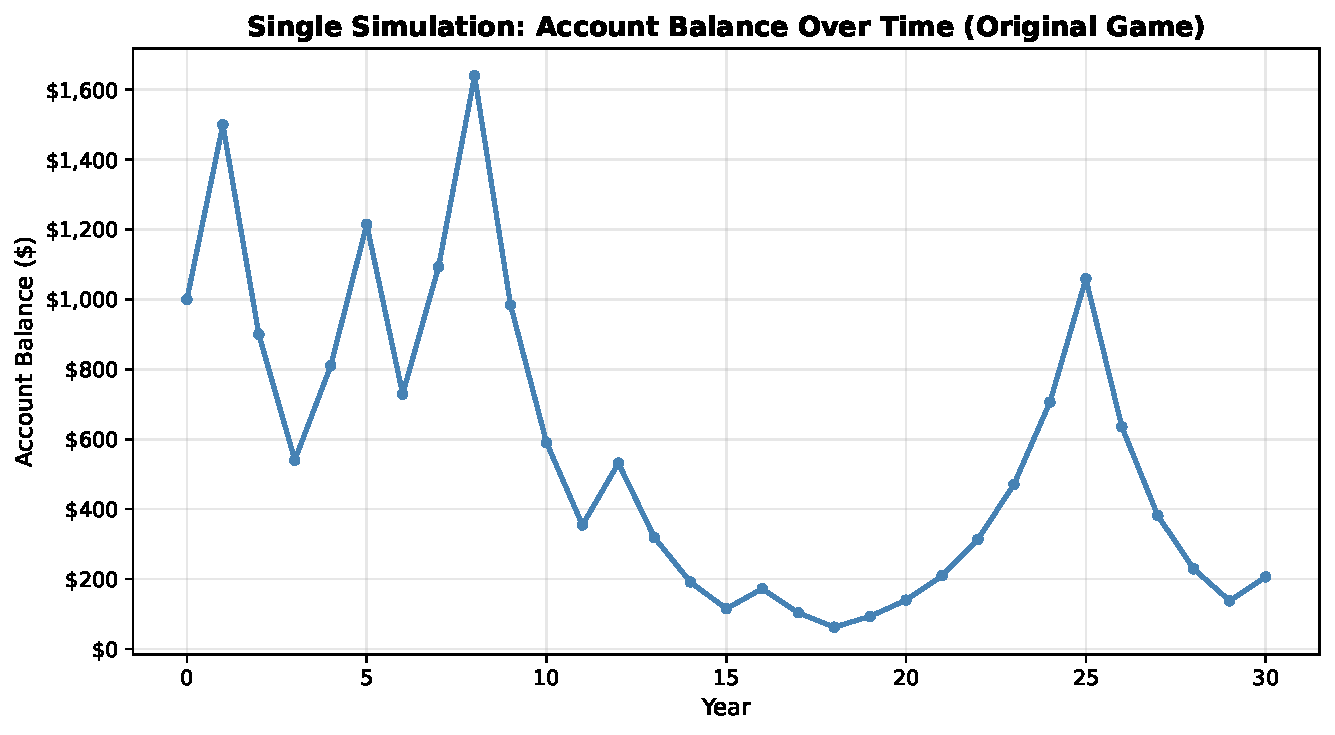
\includegraphics[keepaspectratio]{index_files/figure-pdf/q3-single-simulation-output-1.pdf}}

\begin{verbatim}
Final balance after 30 years: $205.89
\end{verbatim}

\subsubsection{Questions to Answer for 85\% Grade on
Challenge}\label{questions-to-answer-for-85-grade-on-challenge}

\begin{enumerate}
\def\labelenumi{\arabic{enumi}.}
\setcounter{enumi}{3}
\tightlist
\item
  \textbf{Multiple Simulations:} Run 100 simulations modelling the
  dynamics of your account balance over time. Make an object-oriented
  matplotlib OR ggplot2 plot showing a probability distribution of the
  100 simulatedaccount balance at age 55. Comment on the results, are
  you happy? Why or why not?
\end{enumerate}

\subsection{Answer: Below are 100 simulations of the original game over
30 years (age 25 to 55) with a Matplotlib histogram showing the
distribution of final balances. I did buckets for every \$500 and for
any value above \$10,000, I placed it in that bucket. I am not very
happy with the results because there is a 70\% chance that my account
balance by age 55 will be below the \$1,000 threshold. Therefore, I am
not a risky player so there is no point of me trying to play this game
since most likely, I will end up losing money. There is a small chance
to hit the lottery and end up with over \$10,000, but that risk is not
worth it
statistically.}\label{answer-below-are-100-simulations-of-the-original-game-over-30-years-age-25-to-55-with-a-matplotlib-histogram-showing-the-distribution-of-final-balances.-i-did-buckets-for-every-500-and-for-any-value-above-10000-i-placed-it-in-that-bucket.-i-am-not-very-happy-with-the-results-because-there-is-a-70-chance-that-my-account-balance-by-age-55-will-be-below-the-1000-threshold.-therefore-i-am-not-a-risky-player-so-there-is-no-point-of-me-trying-to-play-this-game-since-most-likely-i-will-end-up-losing-money.-there-is-a-small-chance-to-hit-the-lottery-and-end-up-with-over-10000-but-that-risk-is-not-worth-it-statistically.}

\begin{Shaded}
\begin{Highlighting}[]
\ImportTok{import}\NormalTok{ numpy }\ImportTok{as}\NormalTok{ np}
\ImportTok{import}\NormalTok{ matplotlib.pyplot }\ImportTok{as}\NormalTok{ plt}

\CommentTok{\# Reproducibility}
\NormalTok{np.random.seed(}\DecValTok{456}\NormalTok{)}

\CommentTok{\# Parameters (original game rules)}
\NormalTok{initial\_balance }\OperatorTok{=} \FloatTok{1000.0}
\NormalTok{n\_years }\OperatorTok{=} \DecValTok{30}  \CommentTok{\# simulate 30 annual flips (age 25 to 55)}
\NormalTok{n\_sims }\OperatorTok{=} \DecValTok{100}
\NormalTok{p\_heads }\OperatorTok{=} \FloatTok{0.5}

\CommentTok{\# Function to simulate one path}
\KeywordTok{def}\NormalTok{ simulate\_one\_path(initial, years):}
\NormalTok{    balance }\OperatorTok{=}\NormalTok{ initial}
    \ControlFlowTok{for}\NormalTok{ \_ }\KeywordTok{in} \BuiltInTok{range}\NormalTok{(years):}
\NormalTok{        flip }\OperatorTok{=}\NormalTok{ np.random.binomial(}\DecValTok{1}\NormalTok{, p\_heads)}
        \ControlFlowTok{if}\NormalTok{ flip }\OperatorTok{==} \DecValTok{1}\NormalTok{:}
\NormalTok{            balance }\OperatorTok{*=} \FloatTok{1.5}  \CommentTok{\# +50\% on heads}
        \ControlFlowTok{else}\NormalTok{:}
\NormalTok{            balance }\OperatorTok{*=} \FloatTok{0.6}   \CommentTok{\# {-}40\% on tails}
    \ControlFlowTok{return}\NormalTok{ balance}

\CommentTok{\# Run 100 simulations}
\NormalTok{final\_balances }\OperatorTok{=}\NormalTok{ [simulate\_one\_path(initial\_balance, n\_years) }\ControlFlowTok{for}\NormalTok{ \_ }\KeywordTok{in} \BuiltInTok{range}\NormalTok{(n\_sims)]}

\CommentTok{\# OO Matplotlib histogram with custom $500 buckets}
\NormalTok{fig, ax }\OperatorTok{=}\NormalTok{ plt.subplots(figsize}\OperatorTok{=}\NormalTok{(}\DecValTok{14}\NormalTok{, }\DecValTok{8}\NormalTok{))}

\CommentTok{\# Create custom bins every $500, with $10,000+ as final bucket}
\NormalTok{min\_balance }\OperatorTok{=} \BuiltInTok{min}\NormalTok{(final\_balances)}
\NormalTok{max\_balance }\OperatorTok{=} \BuiltInTok{max}\NormalTok{(final\_balances)}
\NormalTok{custom\_bins }\OperatorTok{=} \BuiltInTok{list}\NormalTok{(}\BuiltInTok{range}\NormalTok{(}\DecValTok{0}\NormalTok{, }\DecValTok{10001}\NormalTok{, }\DecValTok{500}\NormalTok{))  }\CommentTok{\# $0, $500, $1000, $1500, ..., $10000}
\ControlFlowTok{if}\NormalTok{ max\_balance }\OperatorTok{\textgreater{}} \DecValTok{10000}\NormalTok{:}
\NormalTok{    custom\_bins.append(max\_balance)  }\CommentTok{\# Add final bin for anything over $10,000}

\NormalTok{n, bins, patches }\OperatorTok{=}\NormalTok{ ax.hist(final\_balances, bins}\OperatorTok{=}\NormalTok{custom\_bins, color}\OperatorTok{=}\StringTok{\textquotesingle{}lightblue\textquotesingle{}}\NormalTok{, alpha}\OperatorTok{=}\FloatTok{0.7}\NormalTok{, edgecolor}\OperatorTok{=}\StringTok{\textquotesingle{}black\textquotesingle{}}\NormalTok{, linewidth}\OperatorTok{=}\FloatTok{0.5}\NormalTok{)}

\CommentTok{\# Color bars based on whether they\textquotesingle{}re above or below $1,000}
\ControlFlowTok{for}\NormalTok{ i, (patch, bin\_left, bin\_right) }\KeywordTok{in} \BuiltInTok{enumerate}\NormalTok{(}\BuiltInTok{zip}\NormalTok{(patches, bins[:}\OperatorTok{{-}}\DecValTok{1}\NormalTok{], bins[}\DecValTok{1}\NormalTok{:])):}
    \ControlFlowTok{if}\NormalTok{ bin\_right }\OperatorTok{\textless{}=}\NormalTok{ initial\_balance:}
\NormalTok{        patch.set\_facecolor(}\StringTok{\textquotesingle{}lightcoral\textquotesingle{}}\NormalTok{)  }\CommentTok{\# Red for below $1,000}
    \ControlFlowTok{else}\NormalTok{:}
\NormalTok{        patch.set\_facecolor(}\StringTok{\textquotesingle{}lightgreen\textquotesingle{}}\NormalTok{)  }\CommentTok{\# Green for above $1,000}

\CommentTok{\# Add vertical line at $1,000}
\NormalTok{ax.axvline(initial\_balance, color}\OperatorTok{=}\StringTok{\textquotesingle{}red\textquotesingle{}}\NormalTok{, linestyle}\OperatorTok{=}\StringTok{\textquotesingle{}{-}{-}\textquotesingle{}}\NormalTok{, linewidth}\OperatorTok{=}\DecValTok{3}\NormalTok{, label}\OperatorTok{=}\SpecialStringTok{f\textquotesingle{}$1,000 Threshold\textquotesingle{}}\NormalTok{)}

\CommentTok{\# Add probability text boxes}
\NormalTok{prob\_above }\OperatorTok{=}\NormalTok{ np.mean(np.array(final\_balances) }\OperatorTok{\textgreater{}}\NormalTok{ initial\_balance)}
\NormalTok{prob\_below }\OperatorTok{=} \DecValTok{1} \OperatorTok{{-}}\NormalTok{ prob\_above}

\NormalTok{ax.text(}\FloatTok{0.02}\NormalTok{, }\FloatTok{0.98}\NormalTok{, }\SpecialStringTok{f\textquotesingle{}Above $1,000: }\SpecialCharTok{\{}\NormalTok{prob\_above}\SpecialCharTok{:.1\%\}}\SpecialStringTok{\textquotesingle{}}\NormalTok{, transform}\OperatorTok{=}\NormalTok{ax.transAxes, }
\NormalTok{        fontsize}\OperatorTok{=}\DecValTok{12}\NormalTok{, fontweight}\OperatorTok{=}\StringTok{\textquotesingle{}bold\textquotesingle{}}\NormalTok{, color}\OperatorTok{=}\StringTok{\textquotesingle{}green\textquotesingle{}}\NormalTok{,}
\NormalTok{        bbox}\OperatorTok{=}\BuiltInTok{dict}\NormalTok{(boxstyle}\OperatorTok{=}\StringTok{\textquotesingle{}round,pad=0.5\textquotesingle{}}\NormalTok{, facecolor}\OperatorTok{=}\StringTok{\textquotesingle{}lightgreen\textquotesingle{}}\NormalTok{, alpha}\OperatorTok{=}\FloatTok{0.8}\NormalTok{),}
\NormalTok{        verticalalignment}\OperatorTok{=}\StringTok{\textquotesingle{}top\textquotesingle{}}\NormalTok{)}

\NormalTok{ax.text(}\FloatTok{0.02}\NormalTok{, }\FloatTok{0.88}\NormalTok{, }\SpecialStringTok{f\textquotesingle{}Below $1,000: }\SpecialCharTok{\{}\NormalTok{prob\_below}\SpecialCharTok{:.1\%\}}\SpecialStringTok{\textquotesingle{}}\NormalTok{, transform}\OperatorTok{=}\NormalTok{ax.transAxes, }
\NormalTok{        fontsize}\OperatorTok{=}\DecValTok{12}\NormalTok{, fontweight}\OperatorTok{=}\StringTok{\textquotesingle{}bold\textquotesingle{}}\NormalTok{, color}\OperatorTok{=}\StringTok{\textquotesingle{}red\textquotesingle{}}\NormalTok{,}
\NormalTok{        bbox}\OperatorTok{=}\BuiltInTok{dict}\NormalTok{(boxstyle}\OperatorTok{=}\StringTok{\textquotesingle{}round,pad=0.5\textquotesingle{}}\NormalTok{, facecolor}\OperatorTok{=}\StringTok{\textquotesingle{}lightcoral\textquotesingle{}}\NormalTok{, alpha}\OperatorTok{=}\FloatTok{0.8}\NormalTok{),}
\NormalTok{        verticalalignment}\OperatorTok{=}\StringTok{\textquotesingle{}top\textquotesingle{}}\NormalTok{)}

\NormalTok{ax.set\_title(}\StringTok{\textquotesingle{}Distribution of Final Account Balances at Age 55}\CharTok{\textbackslash{}n}\StringTok{100 Simulations {-} $500 Buckets (10K+ Grouped)\textquotesingle{}}\NormalTok{, }
\NormalTok{             fontsize}\OperatorTok{=}\DecValTok{14}\NormalTok{, fontweight}\OperatorTok{=}\StringTok{\textquotesingle{}bold\textquotesingle{}}\NormalTok{)}
\NormalTok{ax.set\_xlabel(}\StringTok{\textquotesingle{}Final Balance ($)\textquotesingle{}}\NormalTok{, fontsize}\OperatorTok{=}\DecValTok{12}\NormalTok{)}
\NormalTok{ax.set\_ylabel(}\StringTok{\textquotesingle{}Frequency\textquotesingle{}}\NormalTok{, fontsize}\OperatorTok{=}\DecValTok{12}\NormalTok{)}
\NormalTok{ax.legend()}
\NormalTok{ax.grid(}\VariableTok{True}\NormalTok{, alpha}\OperatorTok{=}\FloatTok{0.3}\NormalTok{)}

\CommentTok{\# Format x{-}axis as currency with $500 increments}
\NormalTok{ax.xaxis.set\_major\_formatter(plt.FuncFormatter(}\KeywordTok{lambda}\NormalTok{ x, \_: }\SpecialStringTok{f\textquotesingle{}$}\SpecialCharTok{\{}\NormalTok{x}\SpecialCharTok{:,.0f\}}\SpecialStringTok{\textquotesingle{}}\NormalTok{))}
\NormalTok{ax.tick\_params(axis}\OperatorTok{=}\StringTok{\textquotesingle{}x\textquotesingle{}}\NormalTok{, rotation}\OperatorTok{=}\DecValTok{45}\NormalTok{)}

\CommentTok{\# Set x{-}axis limits to focus on the main distribution}
\NormalTok{ax.set\_xlim(}\DecValTok{0}\NormalTok{, }\DecValTok{10500}\NormalTok{)}

\NormalTok{plt.tight\_layout()}
\NormalTok{plt.show()}

\CommentTok{\# Summary statistics}
\NormalTok{mean\_balance }\OperatorTok{=}\NormalTok{ np.mean(final\_balances)}
\NormalTok{median\_balance }\OperatorTok{=}\NormalTok{ np.median(final\_balances)}
\NormalTok{prob\_above\_initial }\OperatorTok{=}\NormalTok{ np.mean(np.array(final\_balances) }\OperatorTok{\textgreater{}}\NormalTok{ initial\_balance)}
\NormalTok{max\_balance }\OperatorTok{=}\NormalTok{ np.}\BuiltInTok{max}\NormalTok{(final\_balances)}
\NormalTok{min\_balance }\OperatorTok{=}\NormalTok{ np.}\BuiltInTok{min}\NormalTok{(final\_balances)}

\BuiltInTok{print}\NormalTok{(}\SpecialStringTok{f"Summary Statistics (100 simulations):"}\NormalTok{)}
\BuiltInTok{print}\NormalTok{(}\SpecialStringTok{f"Mean final balance: $}\SpecialCharTok{\{}\NormalTok{mean\_balance}\SpecialCharTok{:,.2f\}}\SpecialStringTok{"}\NormalTok{)}
\BuiltInTok{print}\NormalTok{(}\SpecialStringTok{f"Median final balance: $}\SpecialCharTok{\{}\NormalTok{median\_balance}\SpecialCharTok{:,.2f\}}\SpecialStringTok{"}\NormalTok{)}
\BuiltInTok{print}\NormalTok{(}\SpecialStringTok{f"Probability above $1,000: }\SpecialCharTok{\{}\NormalTok{prob\_above\_initial}\SpecialCharTok{:.3f\}}\SpecialStringTok{"}\NormalTok{)}
\BuiltInTok{print}\NormalTok{(}\SpecialStringTok{f"Maximum balance: $}\SpecialCharTok{\{}\NormalTok{max\_balance}\SpecialCharTok{:,.2f\}}\SpecialStringTok{"}\NormalTok{)}
\BuiltInTok{print}\NormalTok{(}\SpecialStringTok{f"Minimum balance: $}\SpecialCharTok{\{}\NormalTok{min\_balance}\SpecialCharTok{:,.2f\}}\SpecialStringTok{"}\NormalTok{)}
\end{Highlighting}
\end{Shaded}

\pandocbounded{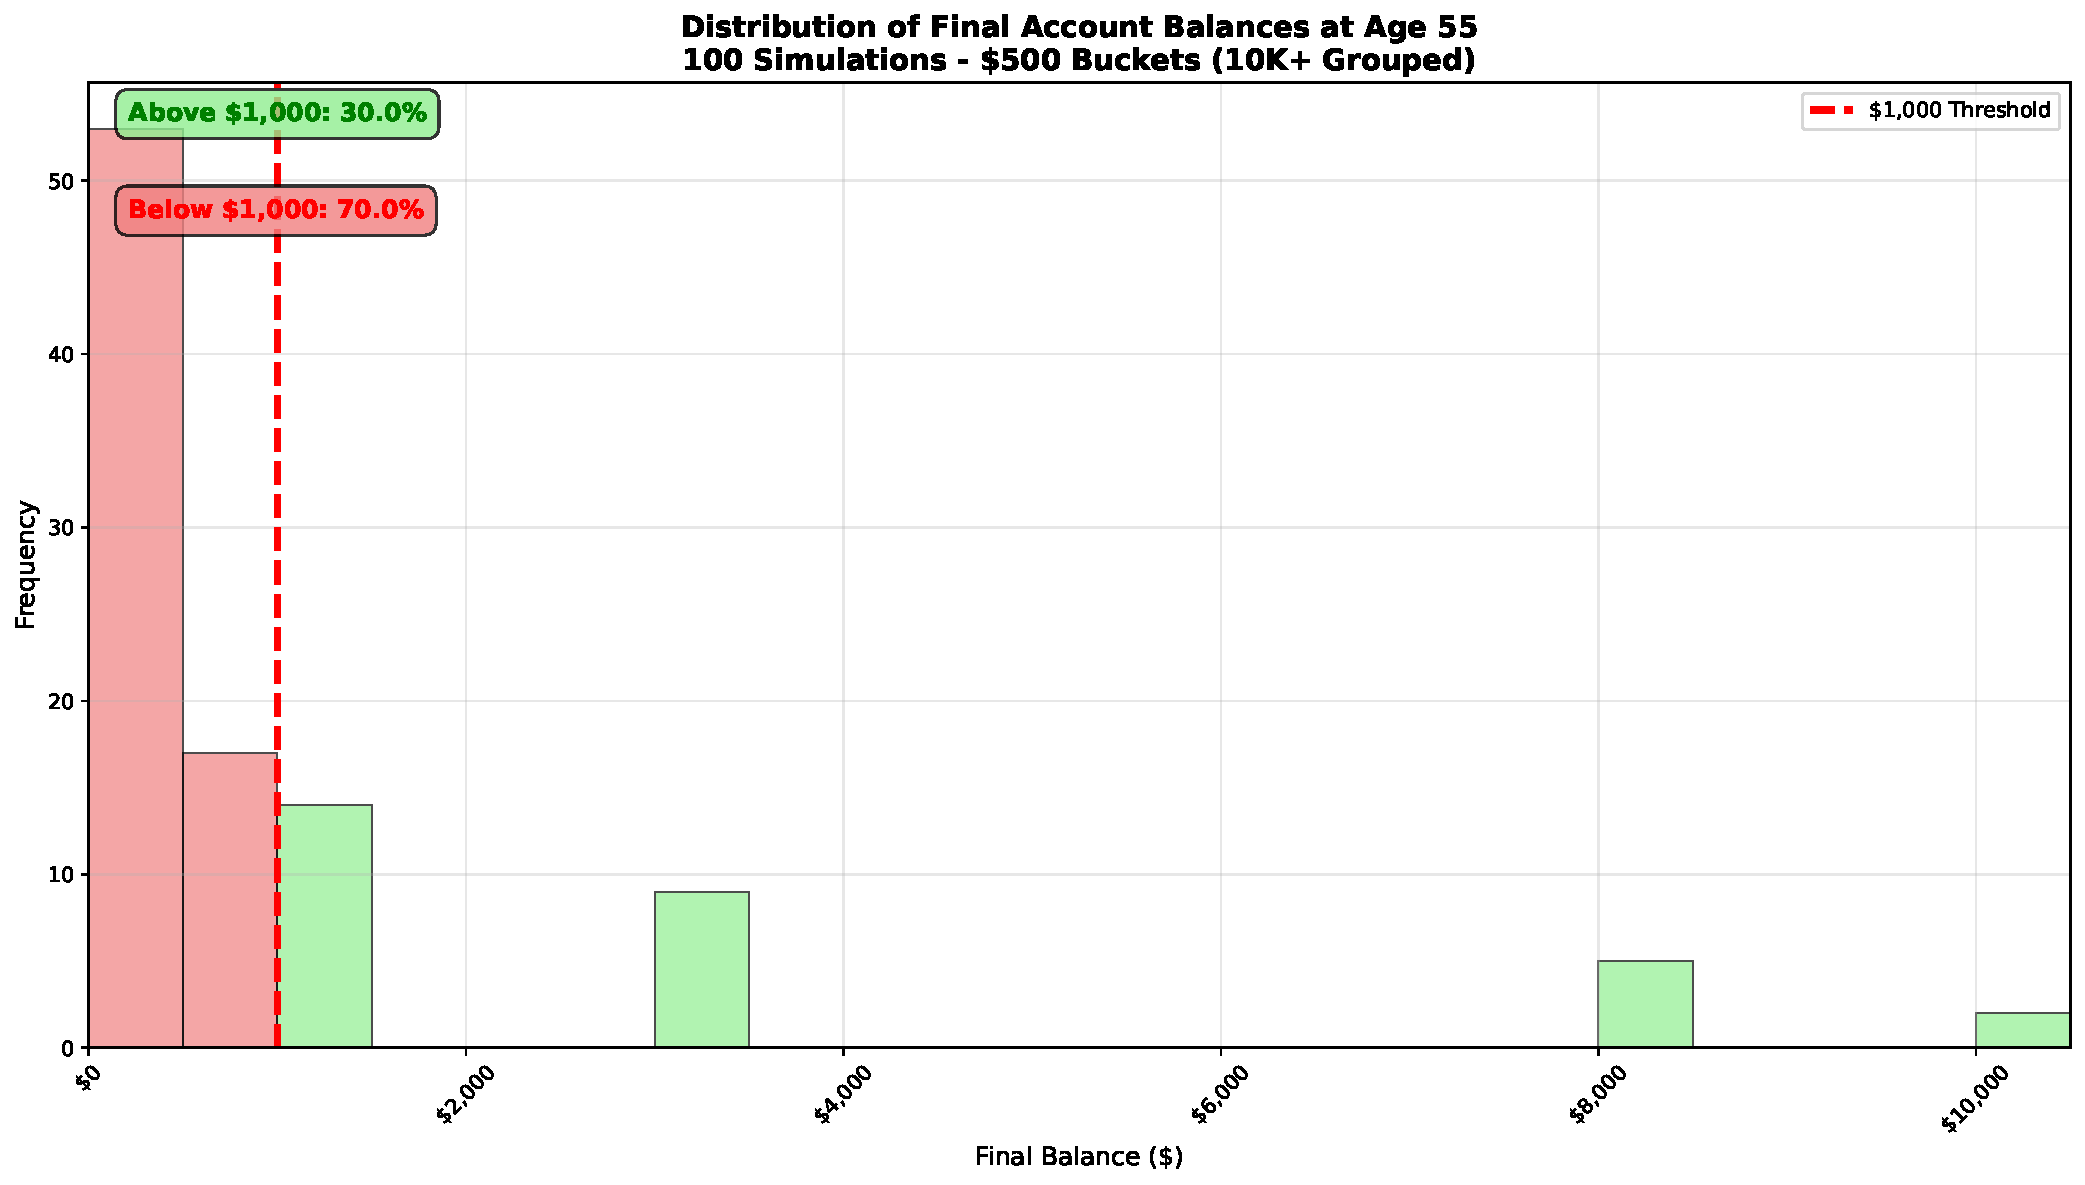
\includegraphics[keepaspectratio]{index_files/figure-pdf/q4-multiple-simulations-output-1.pdf}}

\begin{verbatim}
Summary Statistics (100 simulations):
Mean final balance: $1,718.87
Median final balance: $205.89
Probability above $1,000: 0.300
Maximum balance: $50,266.39
Minimum balance: $0.13
\end{verbatim}

\subsubsection{Questions to Answer for 95\% Grade on
Challenge}\label{questions-to-answer-for-95-grade-on-challenge}

\begin{enumerate}
\def\labelenumi{\arabic{enumi}.}
\setcounter{enumi}{4}
\tightlist
\item
  \textbf{Probability Analysis:} Based on the 100 simulations above,
  what is the probability that your account balance will be greater than
  \$1,000 at age 55?
\end{enumerate}

\subsection{Answer: Based on the 100 simulations from Question 4, the
probability of ending above \$1,000 at age 55 is 30\%. This means that
the probability you end up with less than \$1,000 will be 70\% which is
not a great outcome for the
player.}\label{answer-based-on-the-100-simulations-from-question-4-the-probability-of-ending-above-1000-at-age-55-is-30.-this-means-that-the-probability-you-end-up-with-less-than-1000-will-be-70-which-is-not-a-great-outcome-for-the-player.}

\phantomsection\label{q5-probability-analysis}
\begin{Shaded}
\begin{Highlighting}[]
\CommentTok{\# Use the same final\_balances from Question 4 simulations}
\CommentTok{\# (In practice, you\textquotesingle{}d use the results from the previous simulation)}

\CommentTok{\# Re{-}run the same simulation for consistency}
\ImportTok{import}\NormalTok{ numpy }\ImportTok{as}\NormalTok{ np}

\CommentTok{\# Reproducibility (same seed as Question 4)}
\NormalTok{np.random.seed(}\DecValTok{456}\NormalTok{)}

\CommentTok{\# Parameters (same as Question 4)}
\NormalTok{initial\_balance }\OperatorTok{=} \FloatTok{1000.0}
\NormalTok{n\_years }\OperatorTok{=} \DecValTok{30}
\NormalTok{n\_sims }\OperatorTok{=} \DecValTok{100}
\NormalTok{p\_heads }\OperatorTok{=} \FloatTok{0.5}

\CommentTok{\# Function to simulate one path (same as Question 4)}
\KeywordTok{def}\NormalTok{ simulate\_one\_path(initial, years):}
\NormalTok{    balance }\OperatorTok{=}\NormalTok{ initial}
    \ControlFlowTok{for}\NormalTok{ \_ }\KeywordTok{in} \BuiltInTok{range}\NormalTok{(years):}
\NormalTok{        flip }\OperatorTok{=}\NormalTok{ np.random.binomial(}\DecValTok{1}\NormalTok{, p\_heads)}
        \ControlFlowTok{if}\NormalTok{ flip }\OperatorTok{==} \DecValTok{1}\NormalTok{:}
\NormalTok{            balance }\OperatorTok{*=} \FloatTok{1.5}  \CommentTok{\# +50\% on heads}
        \ControlFlowTok{else}\NormalTok{:}
\NormalTok{            balance }\OperatorTok{*=} \FloatTok{0.6}   \CommentTok{\# {-}40\% on tails}
    \ControlFlowTok{return}\NormalTok{ balance}

\CommentTok{\# Run 100 simulations (same as Question 4)}
\NormalTok{final\_balances }\OperatorTok{=}\NormalTok{ [simulate\_one\_path(initial\_balance, n\_years) }\ControlFlowTok{for}\NormalTok{ \_ }\KeywordTok{in} \BuiltInTok{range}\NormalTok{(n\_sims)]}

\CommentTok{\# Calculate probability of ending above $1,000}
\NormalTok{prob\_above\_1000 }\OperatorTok{=}\NormalTok{ np.mean(np.array(final\_balances) }\OperatorTok{\textgreater{}} \DecValTok{1000}\NormalTok{)}
\NormalTok{prob\_below\_1000 }\OperatorTok{=} \DecValTok{1} \OperatorTok{{-}}\NormalTok{ prob\_above\_1000}

\CommentTok{\# Count actual results}
\NormalTok{count\_above\_1000 }\OperatorTok{=}\NormalTok{ np.}\BuiltInTok{sum}\NormalTok{(np.array(final\_balances) }\OperatorTok{\textgreater{}} \DecValTok{1000}\NormalTok{)}
\NormalTok{count\_below\_1000 }\OperatorTok{=}\NormalTok{ n\_sims }\OperatorTok{{-}}\NormalTok{ count\_above\_1000}

\BuiltInTok{print}\NormalTok{(}\SpecialStringTok{f"Results from 100 simulations:"}\NormalTok{)}
\BuiltInTok{print}\NormalTok{(}\SpecialStringTok{f"Simulations ending above $1,000: }\SpecialCharTok{\{}\NormalTok{count\_above\_1000}\SpecialCharTok{\}}\SpecialStringTok{"}\NormalTok{)}
\BuiltInTok{print}\NormalTok{(}\SpecialStringTok{f"Simulations ending below $1,000: }\SpecialCharTok{\{}\NormalTok{count\_below\_1000}\SpecialCharTok{\}}\SpecialStringTok{"}\NormalTok{)}
\BuiltInTok{print}\NormalTok{(}\SpecialStringTok{f""}\NormalTok{)}
\BuiltInTok{print}\NormalTok{(}\SpecialStringTok{f"Probability of ending above $1,000: }\SpecialCharTok{\{}\NormalTok{prob\_above\_1000}\SpecialCharTok{:.3f\}}\SpecialStringTok{ (}\SpecialCharTok{\{}\NormalTok{prob\_above\_1000}\SpecialCharTok{:.1\%\}}\SpecialStringTok{)"}\NormalTok{)}
\BuiltInTok{print}\NormalTok{(}\SpecialStringTok{f"Probability of ending below $1,000: }\SpecialCharTok{\{}\NormalTok{prob\_below\_1000}\SpecialCharTok{:.3f\}}\SpecialStringTok{ (}\SpecialCharTok{\{}\NormalTok{prob\_below\_1000}\SpecialCharTok{:.1\%\}}\SpecialStringTok{)"}\NormalTok{)}
\BuiltInTok{print}\NormalTok{(}\SpecialStringTok{f""}\NormalTok{)}
\BuiltInTok{print}\NormalTok{(}\SpecialStringTok{f"Answer: The probability that your account balance will be greater than $1,000 at age 55 is }\SpecialCharTok{\{}\NormalTok{prob\_above\_1000}\SpecialCharTok{:.1\%\}}\SpecialStringTok{"}\NormalTok{)}
\end{Highlighting}
\end{Shaded}

\begin{verbatim}
Results from 100 simulations:
Simulations ending above $1,000: 30
Simulations ending below $1,000: 70

Probability of ending above $1,000: 0.300 (30.0%)
Probability of ending below $1,000: 0.700 (70.0%)

Answer: The probability that your account balance will be greater than $1,000 at age 55 is 30.0%
\end{verbatim}

\subsubsection{Questions to Answer for 100\% Grade on
Challenge}\label{questions-to-answer-for-100-grade-on-challenge}

\begin{enumerate}
\def\labelenumi{\arabic{enumi}.}
\setcounter{enumi}{5}
\tightlist
\item
  \textbf{Strategy Comparison:} Run 100 simulations for the modified
  game strategy shown below in
  Example~\ref{exm-ErgodicityEconomicsExampleModified}. What is the
  probability that your account balance will be greater than \$10,000 at
  age 55? Is this probability higher or lower than the probability in
  the original game?
\end{enumerate}

\subsection{Answer: Below are 100 simulations of the modified game
strategy (betting 50\% of balance each round) compared to the original
game. The modified strategy shows different dynamics due to the fixed
betting
percentage.}\label{answer-below-are-100-simulations-of-the-modified-game-strategy-betting-50-of-balance-each-round-compared-to-the-original-game.-the-modified-strategy-shows-different-dynamics-due-to-the-fixed-betting-percentage.}

\begin{Shaded}
\begin{Highlighting}[]
\ImportTok{import}\NormalTok{ numpy }\ImportTok{as}\NormalTok{ np}
\ImportTok{import}\NormalTok{ matplotlib.pyplot }\ImportTok{as}\NormalTok{ plt}

\CommentTok{\# Reproducibility}
\NormalTok{np.random.seed(}\DecValTok{789}\NormalTok{)}

\CommentTok{\# Parameters}
\NormalTok{initial\_balance }\OperatorTok{=} \FloatTok{1000.0}
\NormalTok{n\_years }\OperatorTok{=} \DecValTok{30}
\NormalTok{n\_sims }\OperatorTok{=} \DecValTok{100}
\NormalTok{p\_heads }\OperatorTok{=} \FloatTok{0.5}

\CommentTok{\# Original game function (from Questions 4{-}5)}
\KeywordTok{def}\NormalTok{ simulate\_original\_game(initial, years):}
\NormalTok{    balance }\OperatorTok{=}\NormalTok{ initial}
    \ControlFlowTok{for}\NormalTok{ \_ }\KeywordTok{in} \BuiltInTok{range}\NormalTok{(years):}
\NormalTok{        flip }\OperatorTok{=}\NormalTok{ np.random.binomial(}\DecValTok{1}\NormalTok{, p\_heads)}
        \ControlFlowTok{if}\NormalTok{ flip }\OperatorTok{==} \DecValTok{1}\NormalTok{:}
\NormalTok{            balance }\OperatorTok{*=} \FloatTok{1.5}  \CommentTok{\# +50\% on heads}
        \ControlFlowTok{else}\NormalTok{:}
\NormalTok{            balance }\OperatorTok{*=} \FloatTok{0.6}   \CommentTok{\# {-}40\% on tails}
    \ControlFlowTok{return}\NormalTok{ balance}

\CommentTok{\# Modified game function (betting 50\% of balance each round)}
\KeywordTok{def}\NormalTok{ simulate\_modified\_game(initial, years):}
\NormalTok{    balance }\OperatorTok{=}\NormalTok{ initial}
    \ControlFlowTok{for}\NormalTok{ \_ }\KeywordTok{in} \BuiltInTok{range}\NormalTok{(years):}
\NormalTok{        flip }\OperatorTok{=}\NormalTok{ np.random.binomial(}\DecValTok{1}\NormalTok{, p\_heads)}
\NormalTok{        bet\_amount }\OperatorTok{=}\NormalTok{ balance }\OperatorTok{*} \FloatTok{0.5}  \CommentTok{\# Bet exactly 50\% of current balance}
        
        \ControlFlowTok{if}\NormalTok{ flip }\OperatorTok{==} \DecValTok{1}\NormalTok{:}
            \CommentTok{\# Win: bet increases by 50\%, so total balance = remaining 50\% + bet*1.5}
\NormalTok{            balance }\OperatorTok{=}\NormalTok{ (balance }\OperatorTok{{-}}\NormalTok{ bet\_amount) }\OperatorTok{+}\NormalTok{ (bet\_amount }\OperatorTok{*} \FloatTok{1.5}\NormalTok{)}
        \ControlFlowTok{else}\NormalTok{:}
            \CommentTok{\# Lose: bet decreases by 40\%, so total balance = remaining 50\% + bet*0.6}
\NormalTok{            balance }\OperatorTok{=}\NormalTok{ (balance }\OperatorTok{{-}}\NormalTok{ bet\_amount) }\OperatorTok{+}\NormalTok{ (bet\_amount }\OperatorTok{*} \FloatTok{0.6}\NormalTok{)}
    \ControlFlowTok{return}\NormalTok{ balance}

\CommentTok{\# Run simulations for both strategies}
\NormalTok{original\_balances }\OperatorTok{=}\NormalTok{ [simulate\_original\_game(initial\_balance, n\_years) }\ControlFlowTok{for}\NormalTok{ \_ }\KeywordTok{in} \BuiltInTok{range}\NormalTok{(n\_sims)]}
\NormalTok{modified\_balances }\OperatorTok{=}\NormalTok{ [simulate\_modified\_game(initial\_balance, n\_years) }\ControlFlowTok{for}\NormalTok{ \_ }\KeywordTok{in} \BuiltInTok{range}\NormalTok{(n\_sims)]}

\CommentTok{\# Calculate probabilities}
\NormalTok{prob\_original\_above\_10k }\OperatorTok{=}\NormalTok{ np.mean(np.array(original\_balances) }\OperatorTok{\textgreater{}} \DecValTok{10000}\NormalTok{)}
\NormalTok{prob\_modified\_above\_10k }\OperatorTok{=}\NormalTok{ np.mean(np.array(modified\_balances) }\OperatorTok{\textgreater{}} \DecValTok{10000}\NormalTok{)}

\CommentTok{\# Create comparison histogram}
\NormalTok{fig, (ax1, ax2) }\OperatorTok{=}\NormalTok{ plt.subplots(}\DecValTok{1}\NormalTok{, }\DecValTok{2}\NormalTok{, figsize}\OperatorTok{=}\NormalTok{(}\DecValTok{16}\NormalTok{, }\DecValTok{7}\NormalTok{))}

\CommentTok{\# Original game histogram}
\NormalTok{ax1.hist(original\_balances, bins}\OperatorTok{=}\DecValTok{20}\NormalTok{, color}\OperatorTok{=}\StringTok{\textquotesingle{}lightblue\textquotesingle{}}\NormalTok{, alpha}\OperatorTok{=}\FloatTok{0.7}\NormalTok{, edgecolor}\OperatorTok{=}\StringTok{\textquotesingle{}black\textquotesingle{}}\NormalTok{)}
\NormalTok{ax1.axvline(}\DecValTok{10000}\NormalTok{, color}\OperatorTok{=}\StringTok{\textquotesingle{}red\textquotesingle{}}\NormalTok{, linestyle}\OperatorTok{=}\StringTok{\textquotesingle{}{-}{-}\textquotesingle{}}\NormalTok{, linewidth}\OperatorTok{=}\DecValTok{2}\NormalTok{, label}\OperatorTok{=}\StringTok{\textquotesingle{}$10,000 Threshold\textquotesingle{}}\NormalTok{)}
\NormalTok{ax1.set\_title(}\StringTok{\textquotesingle{}Original Game Strategy}\CharTok{\textbackslash{}n}\StringTok{(Full Balance Multiplicative)\textquotesingle{}}\NormalTok{, fontsize}\OperatorTok{=}\DecValTok{12}\NormalTok{, fontweight}\OperatorTok{=}\StringTok{\textquotesingle{}bold\textquotesingle{}}\NormalTok{)}
\NormalTok{ax1.set\_xlabel(}\StringTok{\textquotesingle{}Final Balance ($)\textquotesingle{}}\NormalTok{, fontsize}\OperatorTok{=}\DecValTok{11}\NormalTok{)}
\NormalTok{ax1.set\_ylabel(}\StringTok{\textquotesingle{}Frequency\textquotesingle{}}\NormalTok{, fontsize}\OperatorTok{=}\DecValTok{11}\NormalTok{)}
\NormalTok{ax1.legend()}
\NormalTok{ax1.grid(}\VariableTok{True}\NormalTok{, alpha}\OperatorTok{=}\FloatTok{0.3}\NormalTok{)}
\NormalTok{ax1.xaxis.set\_major\_formatter(plt.FuncFormatter(}\KeywordTok{lambda}\NormalTok{ x, \_: }\SpecialStringTok{f\textquotesingle{}$}\SpecialCharTok{\{}\NormalTok{x}\SpecialCharTok{:,.0f\}}\SpecialStringTok{\textquotesingle{}}\NormalTok{))}

\CommentTok{\# Modified game histogram}
\NormalTok{ax2.hist(modified\_balances, bins}\OperatorTok{=}\DecValTok{20}\NormalTok{, color}\OperatorTok{=}\StringTok{\textquotesingle{}lightgreen\textquotesingle{}}\NormalTok{, alpha}\OperatorTok{=}\FloatTok{0.7}\NormalTok{, edgecolor}\OperatorTok{=}\StringTok{\textquotesingle{}black\textquotesingle{}}\NormalTok{)}
\NormalTok{ax2.axvline(}\DecValTok{10000}\NormalTok{, color}\OperatorTok{=}\StringTok{\textquotesingle{}red\textquotesingle{}}\NormalTok{, linestyle}\OperatorTok{=}\StringTok{\textquotesingle{}{-}{-}\textquotesingle{}}\NormalTok{, linewidth}\OperatorTok{=}\DecValTok{2}\NormalTok{, label}\OperatorTok{=}\StringTok{\textquotesingle{}$10,000 Threshold\textquotesingle{}}\NormalTok{)}
\NormalTok{ax2.set\_title(}\StringTok{\textquotesingle{}Modified Game Strategy}\CharTok{\textbackslash{}n}\StringTok{(Betting 50}\SpecialCharTok{\% o}\StringTok{f Balance)\textquotesingle{}}\NormalTok{, fontsize}\OperatorTok{=}\DecValTok{12}\NormalTok{, fontweight}\OperatorTok{=}\StringTok{\textquotesingle{}bold\textquotesingle{}}\NormalTok{)}
\NormalTok{ax2.set\_xlabel(}\StringTok{\textquotesingle{}Final Balance ($)\textquotesingle{}}\NormalTok{, fontsize}\OperatorTok{=}\DecValTok{11}\NormalTok{)}
\NormalTok{ax2.set\_ylabel(}\StringTok{\textquotesingle{}Frequency\textquotesingle{}}\NormalTok{, fontsize}\OperatorTok{=}\DecValTok{11}\NormalTok{)}
\NormalTok{ax2.legend()}
\NormalTok{ax2.grid(}\VariableTok{True}\NormalTok{, alpha}\OperatorTok{=}\FloatTok{0.3}\NormalTok{)}
\NormalTok{ax2.xaxis.set\_major\_formatter(plt.FuncFormatter(}\KeywordTok{lambda}\NormalTok{ x, \_: }\SpecialStringTok{f\textquotesingle{}$}\SpecialCharTok{\{}\NormalTok{x}\SpecialCharTok{:,.0f\}}\SpecialStringTok{\textquotesingle{}}\NormalTok{))}

\NormalTok{plt.tight\_layout()}
\NormalTok{plt.show()}

\CommentTok{\# Print results}
\BuiltInTok{print}\NormalTok{(}\StringTok{"Strategy Comparison Results:"}\NormalTok{)}
\BuiltInTok{print}\NormalTok{(}\SpecialStringTok{f"Original Game {-} Probability above $10,000: }\SpecialCharTok{\{}\NormalTok{prob\_original\_above\_10k}\SpecialCharTok{:.3f\}}\SpecialStringTok{ (}\SpecialCharTok{\{}\NormalTok{prob\_original\_above\_10k}\SpecialCharTok{:.1\%\}}\SpecialStringTok{)"}\NormalTok{)}
\BuiltInTok{print}\NormalTok{(}\SpecialStringTok{f"Modified Game {-} Probability above $10,000: }\SpecialCharTok{\{}\NormalTok{prob\_modified\_above\_10k}\SpecialCharTok{:.3f\}}\SpecialStringTok{ (}\SpecialCharTok{\{}\NormalTok{prob\_modified\_above\_10k}\SpecialCharTok{:.1\%\}}\SpecialStringTok{)"}\NormalTok{)}
\BuiltInTok{print}\NormalTok{(}\SpecialStringTok{f""}\NormalTok{)}
\BuiltInTok{print}\NormalTok{(}\SpecialStringTok{f"Answer: The probability of ending above $10,000 is }\SpecialCharTok{\{}\NormalTok{prob\_modified\_above\_10k}\SpecialCharTok{:.1\%\}}\SpecialStringTok{ for the modified game."}\NormalTok{)}
\BuiltInTok{print}\NormalTok{(}\SpecialStringTok{f"This is }\SpecialCharTok{\{}\StringTok{\textquotesingle{}HIGHER\textquotesingle{}} \ControlFlowTok{if}\NormalTok{ prob\_modified\_above\_10k }\OperatorTok{\textgreater{}}\NormalTok{ prob\_original\_above\_10k }\ControlFlowTok{else} \StringTok{\textquotesingle{}LOWER\textquotesingle{}}\SpecialCharTok{\}}\SpecialStringTok{ than the original game (}\SpecialCharTok{\{}\NormalTok{prob\_original\_above\_10k}\SpecialCharTok{:.1\%\}}\SpecialStringTok{)."}\NormalTok{)}
\end{Highlighting}
\end{Shaded}

\pandocbounded{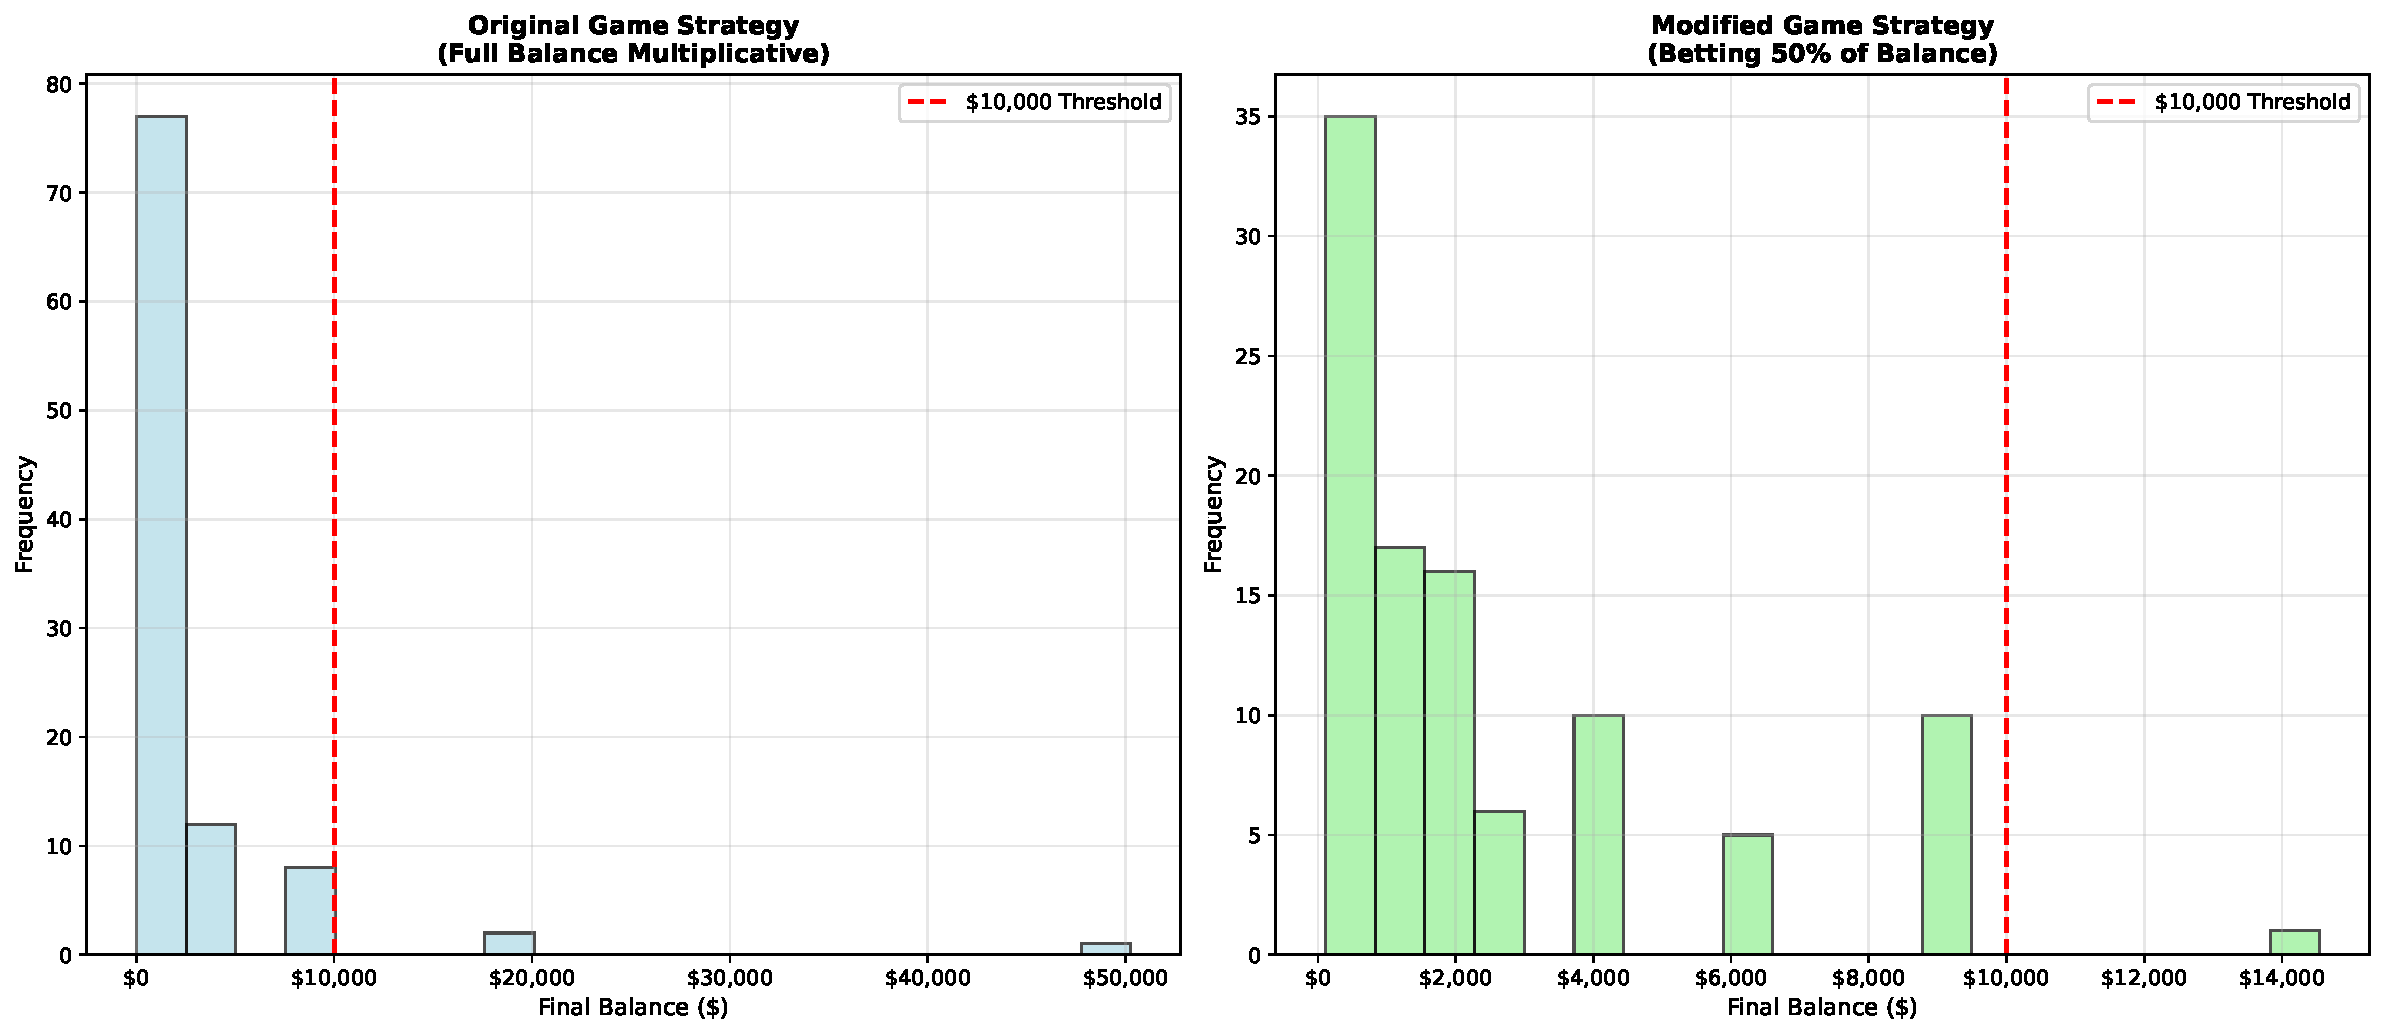
\includegraphics[keepaspectratio]{index_files/figure-pdf/q6-strategy-comparison-output-1.pdf}}

\begin{verbatim}
Strategy Comparison Results:
Original Game - Probability above $10,000: 0.030 (3.0%)
Modified Game - Probability above $10,000: 0.010 (1.0%)

Answer: The probability of ending above $10,000 is 1.0% for the modified game.
This is LOWER than the original game (3.0%).
\end{verbatim}

\subsubsection{Modified Game Strategy}\label{modified-game-strategy}

\begin{example}[]\protect\hypertarget{exm-ErgodicityEconomicsExampleModified}{}\label{exm-ErgodicityEconomicsExampleModified}

Imagine you are offered the following game and given a \$1,000 budget in
a special account to play the game: I will flip a coin, and if it comes
up heads, we increase your bet by 50\%; if it comes up tails, we reduce
your bet by 40\%. You must bet exactly 50\% of your current account
balance on each flip, and this 50\% is locked in for each round. We are
not only doing this once, but we will do it once per year until you turn
55. When you turn 55, you will receive the balance in your account.

\end{example}

\subsection{Technical Implementation Preferences
💡}\label{technical-implementation-preferences}

\subsubsection{Setting Up Your Analysis}\label{setting-up-your-analysis}

\textbf{For R Users:}

\begin{itemize}
\tightlist
\item
  Use \texttt{tidyverse} for data manipulation
\item
  Use \texttt{ggplot2} for visualizations
\item
  Use \texttt{set.seed()} for reproducible results
\end{itemize}

\textbf{For Python Users:}

\begin{itemize}
\tightlist
\item
  Use \texttt{numpy} for numerical operations
\item
  Use \texttt{pandas} for data manipulation
\item
  Use \texttt{matplotlib} (object-oriented)
\item
  Use \texttt{np.random.seed()} for reproducible results
\end{itemize}

\subsubsection{Visualization
Preferences}\label{visualization-preferences}

\begin{itemize}
\tightlist
\item
  \textbf{Professional Styling:} Use consistent colors, clear labels,
  readable fonts, and informative titles
\end{itemize}

\subsection{Submission Checklist ✅}\label{submission-checklist}

\textbf{Minimum Requirements (Required for Any Points):}

\begin{itemize}
\tightlist
\item[$\square$]
  Quarto document created with clear narrative
\item[$\square$]
  Document rendered to HTML successfully
\item[$\square$]
  Repository ``simulationChallenge'' created
\item[$\square$]
  HTML files uploaded to repository
\item[$\square$]
  GitHub Pages enabled and working
\item[$\square$]
  Site accessible at
  \texttt{https://{[}your-username{]}.github.io/simulationChallenge/}
\end{itemize}

\textbf{75\% Grade Requirements:}

\begin{itemize}
\tightlist
\item[$\square$]
  Expected value calculations shown (Question 1)
\item[$\square$]
  Expectation vs.~reality analysis (Question 2)
\item[$\square$]
  Single simulation with time series plot (Question 3)
\item[$\square$]
  Clear interpretation of single simulation results
\end{itemize}

\textbf{85\% Grade Requirements:}

\begin{itemize}
\tightlist
\item[$\square$]
  100 simulations with distribution analysis (Question 4)
\item[$\square$]
  Probability distribution plot of final account balances
\item[$\square$]
  Clear interpretation of multiple simulation results
\end{itemize}

\textbf{95\% Grade Requirements:}

\begin{itemize}
\tightlist
\item[$\square$]
  Probability calculations for original strategy (Question 5)
\item[$\square$]
  Analysis of probability that balance \textgreater{} \$1,000 at age 55
\end{itemize}

\textbf{100\% Grade Requirements:}

\begin{itemize}
\tightlist
\item[$\square$]
  100 simulations for modified strategy (Question 6)
\item[$\square$]
  Probability calculations for modified strategy
\item[$\square$]
  Comparative analysis between both strategies
\item[$\square$]
  Analysis of probability that balance \textgreater{} \$10,000 at age 55
\end{itemize}

\textbf{Code Quality (All Grades):}

\begin{itemize}
\tightlist
\item[$\square$]
  Reproducible results (seeds set)
\item[$\square$]
  Clean, well-commented code
\item[$\square$]
  Appropriate use of functions and loops
\item[$\square$]
  Professional visualization styling
\end{itemize}

\subsubsection{Resources}\label{resources}

\begin{itemize}
\tightlist
\item
  \textbf{Quarto Markdown:}
  \href{https://quarto.org/docs/authoring/markdown-basics.html}{quarto.org/docs/authoring/markdown-basics.html}
\item
  \textbf{Quarto Documentation:}
  \href{https://quarto.org/docs}{quarto.org/docs}
\item
  \textbf{R for Data Science:}
  \href{https://r4ds.had.co.nz}{r4ds.had.co.nz}
\item
  \textbf{Python Data Science Handbook:}
  \href{https://jakevdp.github.io/PythonDataScienceHandbook}{jakevdp.github.io/PythonDataScienceHandbook}
\end{itemize}

\subsubsection{Getting Started Tips}\label{getting-started-tips}

\begin{tcolorbox}[enhanced jigsaw, rightrule=.15mm, leftrule=.75mm, toptitle=1mm, bottomtitle=1mm, title=\textcolor{quarto-callout-note-color}{\faInfo}\hspace{0.5em}{🎯 Navy SEALs Motto}, opacityback=0, colbacktitle=quarto-callout-note-color!10!white, arc=.35mm, coltitle=black, colback=white, breakable, titlerule=0mm, colframe=quarto-callout-note-color-frame, toprule=.15mm, bottomrule=.15mm, left=2mm, opacitybacktitle=0.6]

\begin{quote}
``Slow is Smooth and Smooth is Fast''
\end{quote}

\emph{Take your time to understand the simulation mechanics, plan your
approach carefully, and execute with precision. Rushing through this
challenge will only lead to errors and confusion.}

\end{tcolorbox}

\begin{itemize}
\tightlist
\item
  \textbf{Browse \href{@sec-simulation-concepts}{Essential Simulation
  Concepts}:} This section will give you a good understanding of the
  concepts you need to know to complete the challenge.
\item
  \textbf{Start Simple:} Begin with a single simulation to understand
  the mechanics
\item
  \textbf{Document Everything:} Explain your reasoning and interpret
  your results
\item
  \textbf{Forgetting to Set Seeds:} Always set random seeds for
  reproducible results
\item
  \textbf{Total time to complete:} \textasciitilde3-4 hours for the
  100\% grade ⏱️
\item
  \textbf{Good luck, and remember simulation will steer you right even
  when intuition will steer you wrong!} 🎲
\end{itemize}

\begin{tcolorbox}[enhanced jigsaw, rightrule=.15mm, leftrule=.75mm, toptitle=1mm, bottomtitle=1mm, title=\textcolor{quarto-callout-warning-color}{\faExclamationTriangle}\hspace{0.5em}{💾 Important: Save Your Work Frequently!}, opacityback=0, colbacktitle=quarto-callout-warning-color!10!white, arc=.35mm, coltitle=black, colback=white, breakable, titlerule=0mm, colframe=quarto-callout-warning-color-frame, toprule=.15mm, bottomrule=.15mm, left=2mm, opacitybacktitle=0.6]

\textbf{Before you start coding:} Make sure to commit your work often
using the Source Control panel in Cursor (Ctrl+Shift+G or Cmd+Shift+G).
This prevents the AI from overwriting your progress and ensures you
don't lose your work.

\textbf{Commit after each major step:}

\begin{itemize}
\tightlist
\item
  After completing each simulation example
\item
  After finishing each challenge question
\item
  Before asking the AI for help with new code
\end{itemize}

\textbf{How to commit:}

\begin{enumerate}
\def\labelenumi{\arabic{enumi}.}
\tightlist
\item
  Open Source Control panel (Ctrl+Shift+G)
\item
  Stage your changes (+ button)
\item
  Write a descriptive commit message
\item
  Click the checkmark to commit
\end{enumerate}

\emph{Remember: Frequent commits are your safety net!}

\end{tcolorbox}

\subsection{Essential Simulation Concepts
🎯}\label{sec-simulation-concepts}

Before diving into the challenge, let's review the key simulation
concepts you'll need. These examples will prepare you for the investment
game analysis.

\subsubsection{1. Simple Simulation: Coin Flip
Game}\label{simple-simulation-coin-flip-game}

Let's start with a basic coin flip simulation to understand the
mechanics:

\paragraph{Generative DAG Model for the Simple Coin Flip
Game}\label{generative-dag-model-for-the-simple-coin-flip-game}

\textbf{Key Difference from Investment Game:} Unlike the investment game
DAG (\textbf{?@fig-investment-dag}) which models wealth evolution over
multiple time periods with multiplicative changes, this simple coin flip
DAG represents a single-period game with additive winnings. The
investment game shows how wealth compounds over time
(\(W_t = 1.5 \times W_{t-1}\) or \(W_t = 0.6 \times W_{t-1}\)), while
this simple game shows fixed winnings (\(W = +100\) or \(W = -100\))
based on a single coin flip outcome.

\subsubsection{Python}

\begin{Shaded}
\begin{Highlighting}[]
\ImportTok{import}\NormalTok{ numpy }\ImportTok{as}\NormalTok{ np}
\ImportTok{import}\NormalTok{ pandas }\ImportTok{as}\NormalTok{ pd}

\CommentTok{\# Set seed for reproducibility}
\NormalTok{np.random.seed(}\DecValTok{123}\NormalTok{)}

\CommentTok{\# Number of simulations}
\NormalTok{n\_sims }\OperatorTok{=} \DecValTok{10}

\CommentTok{\# Step 1: Draw coin flips (stochastic node)}
\NormalTok{X }\OperatorTok{=}\NormalTok{ np.random.binomial(n}\OperatorTok{=}\DecValTok{1}\NormalTok{, p}\OperatorTok{=}\FloatTok{0.5}\NormalTok{, size}\OperatorTok{=}\NormalTok{n\_sims)}

\CommentTok{\# Step 2: Compute winnings (deterministic node)}
\NormalTok{W }\OperatorTok{=}\NormalTok{ np.where(X }\OperatorTok{==} \DecValTok{1}\NormalTok{, }\DecValTok{100}\NormalTok{, }\OperatorTok{{-}}\DecValTok{100}\NormalTok{)}

\CommentTok{\# Combine into data frame}
\NormalTok{sim\_data }\OperatorTok{=}\NormalTok{ pd.DataFrame(\{}
    \StringTok{\textquotesingle{}sim\_num\textquotesingle{}}\NormalTok{: }\BuiltInTok{range}\NormalTok{(}\DecValTok{1}\NormalTok{, n\_sims }\OperatorTok{+} \DecValTok{1}\NormalTok{),}
    \StringTok{\textquotesingle{}coin\_flip\textquotesingle{}}\NormalTok{: X,}
    \StringTok{\textquotesingle{}winnings\textquotesingle{}}\NormalTok{: W}
\NormalTok{\})}

\CommentTok{\# Display results}
\NormalTok{sim\_data}
\end{Highlighting}
\end{Shaded}

\phantomsection\label{simple-sim-python}
\begin{longtable}[]{@{}llll@{}}
\toprule\noalign{}
& sim\_num & coin\_flip & winnings \\
\midrule\noalign{}
\endhead
\bottomrule\noalign{}
\endlastfoot
0 & 1 & 1 & 100 \\
1 & 2 & 0 & -100 \\
2 & 3 & 0 & -100 \\
3 & 4 & 1 & 100 \\
4 & 5 & 1 & 100 \\
5 & 6 & 0 & -100 \\
6 & 7 & 1 & 100 \\
7 & 8 & 1 & 100 \\
8 & 9 & 0 & -100 \\
9 & 10 & 0 & -100 \\
\end{longtable}

Python simulation of coin flip game

\subsubsection{2. Time-Series Simulation: Account Balance Over
Time}\label{time-series-simulation-account-balance-over-time}

Now let's simulate how an account balance changes over multiple periods:

\paragraph{Generative DAG Model for Time-Series Account
Balance}\label{generative-dag-model-for-time-series-account-balance}

\textbf{Key Difference from Simple Coin Flip Game:} Unlike the simple
coin flip DAG (\textbf{?@fig-simple-coin-dag}) which represents a
single-period game, this time-series DAG models sequential balance
evolution over multiple periods. Each period's balance depends on the
previous period's balance plus the current coin flip outcome. The simple
game shows independent winnings per flip, while this model shows
cumulative balance changes where \(B_t = B_{t-1} + \Delta_t\) and
\(\Delta_t = +100\) or \(-100\) based on the coin flip.

\subsubsection{Python}

\begin{Shaded}
\begin{Highlighting}[]
\ImportTok{import}\NormalTok{ numpy }\ImportTok{as}\NormalTok{ np}
\ImportTok{import}\NormalTok{ pandas }\ImportTok{as}\NormalTok{ pd}
\ImportTok{import}\NormalTok{ matplotlib.pyplot }\ImportTok{as}\NormalTok{ plt}

\CommentTok{\# Set seed for reproducibility}
\NormalTok{np.random.seed(}\DecValTok{456}\NormalTok{)}

\CommentTok{\# Parameters}
\NormalTok{initial\_balance }\OperatorTok{=} \DecValTok{1000}
\NormalTok{n\_periods }\OperatorTok{=} \DecValTok{10}
\NormalTok{n\_sims }\OperatorTok{=} \DecValTok{1}  \CommentTok{\# Start with one simulation}

\CommentTok{\# Simulate one path}
\KeywordTok{def}\NormalTok{ simulate\_path(initial, periods):}
\NormalTok{    balance }\OperatorTok{=}\NormalTok{ initial}
\NormalTok{    path }\OperatorTok{=}\NormalTok{ [initial]}
    
    \ControlFlowTok{for}\NormalTok{ i }\KeywordTok{in} \BuiltInTok{range}\NormalTok{(periods):}
\NormalTok{        coin\_flip }\OperatorTok{=}\NormalTok{ np.random.binomial(}\DecValTok{1}\NormalTok{, }\FloatTok{0.5}\NormalTok{)}
        \ControlFlowTok{if}\NormalTok{ coin\_flip }\OperatorTok{==} \DecValTok{1}\NormalTok{:}
\NormalTok{            balance }\OperatorTok{=}\NormalTok{ balance }\OperatorTok{+} \DecValTok{100}  \CommentTok{\# $100 gain}
        \ControlFlowTok{else}\NormalTok{:}
\NormalTok{            balance }\OperatorTok{=}\NormalTok{ balance }\OperatorTok{{-}} \DecValTok{100}  \CommentTok{\# $100 loss}
\NormalTok{        path.append(balance)}
    
    \ControlFlowTok{return}\NormalTok{ path}

\CommentTok{\# Run simulation}
\NormalTok{time\_series\_data }\OperatorTok{=}\NormalTok{ pd.DataFrame(\{}
    \StringTok{\textquotesingle{}period\textquotesingle{}}\NormalTok{: }\BuiltInTok{range}\NormalTok{(n\_periods }\OperatorTok{+} \DecValTok{1}\NormalTok{),}
    \StringTok{\textquotesingle{}balance\textquotesingle{}}\NormalTok{: simulate\_path(initial\_balance, n\_periods)}
\NormalTok{\})}

\CommentTok{\# Create time series plot}
\NormalTok{fig, ax }\OperatorTok{=}\NormalTok{ plt.subplots(figsize}\OperatorTok{=}\NormalTok{(}\DecValTok{10}\NormalTok{, }\DecValTok{6}\NormalTok{))}
\NormalTok{ax.plot(time\_series\_data[}\StringTok{\textquotesingle{}period\textquotesingle{}}\NormalTok{], time\_series\_data[}\StringTok{\textquotesingle{}balance\textquotesingle{}}\NormalTok{], }
\NormalTok{        color}\OperatorTok{=}\StringTok{\textquotesingle{}cadetblue\textquotesingle{}}\NormalTok{, linewidth}\OperatorTok{=}\DecValTok{2}\NormalTok{, marker}\OperatorTok{=}\StringTok{\textquotesingle{}o\textquotesingle{}}\NormalTok{, markersize}\OperatorTok{=}\DecValTok{6}\NormalTok{)}
\NormalTok{ax.set\_title(}\StringTok{\textquotesingle{}Account Balance Over Time}\CharTok{\textbackslash{}n}\StringTok{Single Simulation Path\textquotesingle{}}\NormalTok{, }
\NormalTok{             fontsize}\OperatorTok{=}\DecValTok{14}\NormalTok{, fontweight}\OperatorTok{=}\StringTok{\textquotesingle{}bold\textquotesingle{}}\NormalTok{)}
\NormalTok{ax.set\_xlabel(}\StringTok{\textquotesingle{}Period\textquotesingle{}}\NormalTok{, fontsize}\OperatorTok{=}\DecValTok{12}\NormalTok{)}
\NormalTok{ax.set\_ylabel(}\StringTok{\textquotesingle{}Account Balance ($)\textquotesingle{}}\NormalTok{, fontsize}\OperatorTok{=}\DecValTok{12}\NormalTok{)}
\NormalTok{ax.grid(}\VariableTok{True}\NormalTok{, alpha}\OperatorTok{=}\FloatTok{0.3}\NormalTok{)}
\NormalTok{ax.set\_ylim(}\DecValTok{0}\NormalTok{, }\BuiltInTok{max}\NormalTok{(time\_series\_data[}\StringTok{\textquotesingle{}balance\textquotesingle{}}\NormalTok{]) }\OperatorTok{*} \FloatTok{1.1}\NormalTok{)}

\CommentTok{\# Format y{-}axis as currency}
\NormalTok{ax.yaxis.set\_major\_formatter(plt.FuncFormatter(}\KeywordTok{lambda}\NormalTok{ x, p: }\SpecialStringTok{f\textquotesingle{}$}\SpecialCharTok{\{}\NormalTok{x}\SpecialCharTok{:,.0f\}}\SpecialStringTok{\textquotesingle{}}\NormalTok{))}

\NormalTok{plt.tight\_layout()}
\NormalTok{plt.show()}

\CommentTok{\# Show the data}
\BuiltInTok{print}\NormalTok{(}\StringTok{"Time Series Data:"}\NormalTok{)}
\BuiltInTok{print}\NormalTok{(time\_series\_data)}
\end{Highlighting}
\end{Shaded}

\begin{figure}[H]

{\centering \pandocbounded{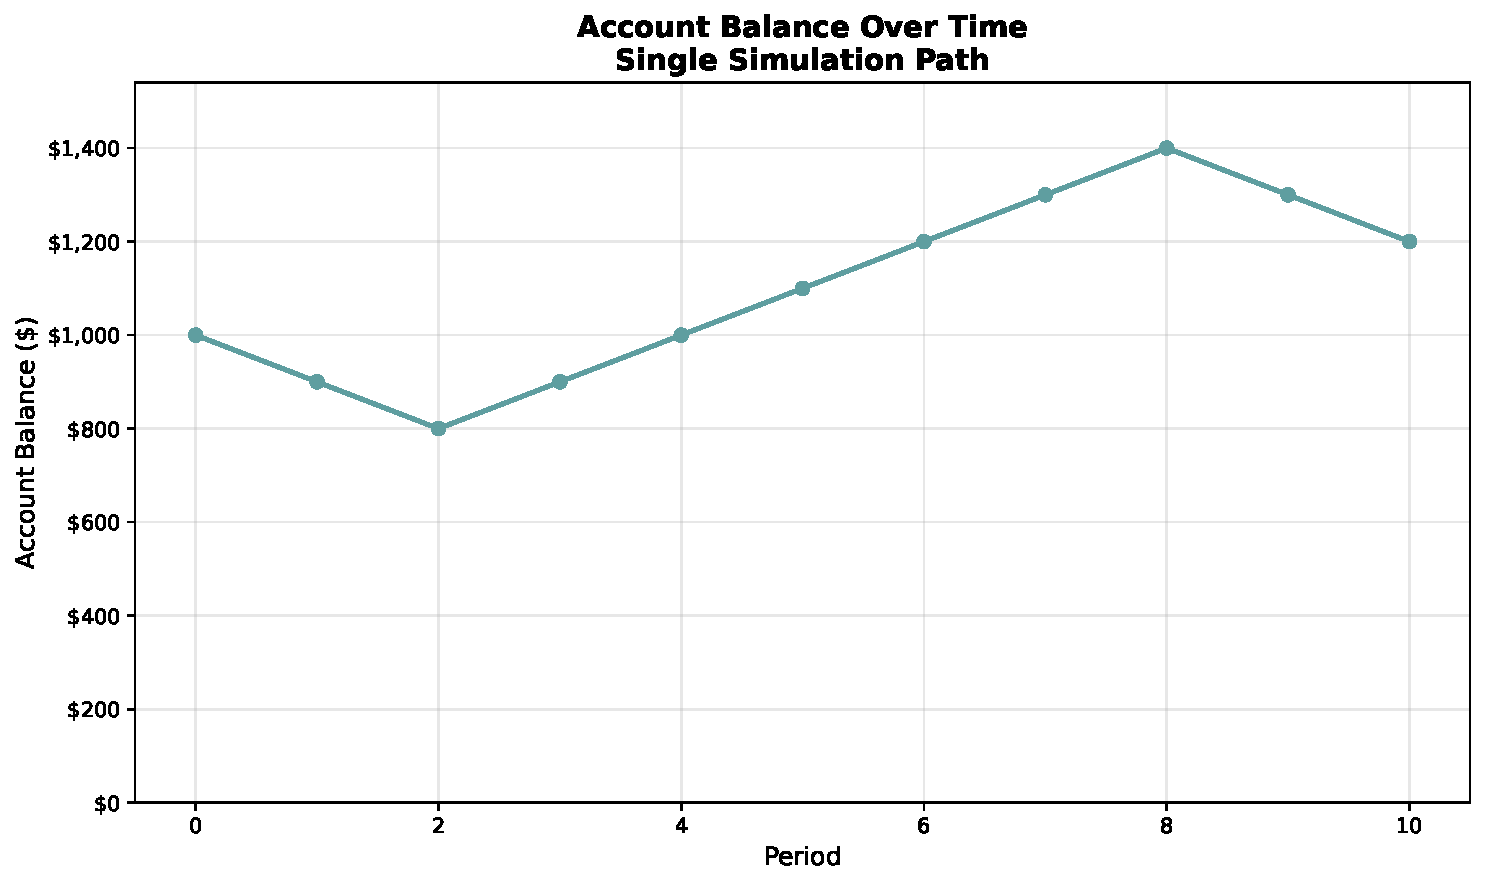
\includegraphics[keepaspectratio]{index_files/figure-pdf/timeseries-sim-python-output-1.pdf}}

}

\caption{Python time-series simulation of account balance}

\end{figure}%

\begin{verbatim}
Time Series Data:
    period  balance
0        0     1000
1        1      900
2        2      800
3        3      900
4        4     1000
5        5     1100
6        6     1200
7        7     1300
8        8     1400
9        9     1300
10      10     1200
\end{verbatim}

\subsubsection{3. Probability Distribution: Final Balance
Distribution}\label{probability-distribution-final-balance-distribution}

Let's see what the distribution of final balances looks like across many
simulations:

\subsubsection{Python}

\begin{Shaded}
\begin{Highlighting}[]
\ImportTok{import}\NormalTok{ numpy }\ImportTok{as}\NormalTok{ np}
\ImportTok{import}\NormalTok{ pandas }\ImportTok{as}\NormalTok{ pd}
\ImportTok{import}\NormalTok{ matplotlib.pyplot }\ImportTok{as}\NormalTok{ plt}

\CommentTok{\# Set seed for reproducibility}
\NormalTok{np.random.seed(}\DecValTok{789}\NormalTok{)}

\CommentTok{\# Parameters}
\NormalTok{initial\_balance }\OperatorTok{=} \DecValTok{1000}
\NormalTok{n\_periods }\OperatorTok{=} \DecValTok{10}
\NormalTok{n\_sims }\OperatorTok{=} \DecValTok{100}  \CommentTok{\# Multiple simulations}

\CommentTok{\# Simulate multiple paths}
\KeywordTok{def}\NormalTok{ simulate\_final\_balance(initial, periods):}
\NormalTok{    balance }\OperatorTok{=}\NormalTok{ initial}
    \ControlFlowTok{for}\NormalTok{ i }\KeywordTok{in} \BuiltInTok{range}\NormalTok{(periods):}
\NormalTok{        coin\_flip }\OperatorTok{=}\NormalTok{ np.random.binomial(}\DecValTok{1}\NormalTok{, }\FloatTok{0.5}\NormalTok{)}
        \ControlFlowTok{if}\NormalTok{ coin\_flip }\OperatorTok{==} \DecValTok{1}\NormalTok{:}
\NormalTok{            balance }\OperatorTok{=}\NormalTok{ balance }\OperatorTok{+} \DecValTok{100}  \CommentTok{\# $100 gain}
        \ControlFlowTok{else}\NormalTok{:}
\NormalTok{            balance }\OperatorTok{=}\NormalTok{ balance }\OperatorTok{{-}} \DecValTok{100}  \CommentTok{\# $100 loss}
    \ControlFlowTok{return}\NormalTok{ balance}

\CommentTok{\# Run multiple simulations}
\NormalTok{final\_balances }\OperatorTok{=}\NormalTok{ [simulate\_final\_balance(initial\_balance, n\_periods) }\ControlFlowTok{for}\NormalTok{ \_ }\KeywordTok{in} \BuiltInTok{range}\NormalTok{(n\_sims)]}

\CommentTok{\# Create data frame}
\NormalTok{distribution\_data }\OperatorTok{=}\NormalTok{ pd.DataFrame(\{}
    \StringTok{\textquotesingle{}sim\_num\textquotesingle{}}\NormalTok{: }\BuiltInTok{range}\NormalTok{(}\DecValTok{1}\NormalTok{, n\_sims }\OperatorTok{+} \DecValTok{1}\NormalTok{),}
    \StringTok{\textquotesingle{}final\_balance\textquotesingle{}}\NormalTok{: final\_balances}
\NormalTok{\})}

\CommentTok{\# Create histogram}
\NormalTok{fig, ax }\OperatorTok{=}\NormalTok{ plt.subplots(figsize}\OperatorTok{=}\NormalTok{(}\DecValTok{10}\NormalTok{, }\DecValTok{6}\NormalTok{))}
\NormalTok{ax.hist(distribution\_data[}\StringTok{\textquotesingle{}final\_balance\textquotesingle{}}\NormalTok{], bins}\OperatorTok{=}\DecValTok{20}\NormalTok{, color}\OperatorTok{=}\StringTok{\textquotesingle{}plum\textquotesingle{}}\NormalTok{, alpha}\OperatorTok{=}\FloatTok{0.8}\NormalTok{, edgecolor}\OperatorTok{=}\StringTok{\textquotesingle{}black\textquotesingle{}}\NormalTok{)}
\NormalTok{ax.axvline(initial\_balance, color}\OperatorTok{=}\StringTok{\textquotesingle{}red\textquotesingle{}}\NormalTok{, linestyle}\OperatorTok{=}\StringTok{\textquotesingle{}{-}{-}\textquotesingle{}}\NormalTok{, linewidth}\OperatorTok{=}\DecValTok{2}\NormalTok{, label}\OperatorTok{=}\StringTok{\textquotesingle{}Initial Balance\textquotesingle{}}\NormalTok{)}
\NormalTok{ax.set\_title(}\SpecialStringTok{f\textquotesingle{}Distribution of Final Account Balances}\CharTok{\textbackslash{}n}\SpecialStringTok{100 Simulations, }\SpecialCharTok{\{}\NormalTok{n\_periods}\SpecialCharTok{\}}\SpecialStringTok{ Periods Each\textquotesingle{}}\NormalTok{, }
\NormalTok{             fontsize}\OperatorTok{=}\DecValTok{14}\NormalTok{, fontweight}\OperatorTok{=}\StringTok{\textquotesingle{}bold\textquotesingle{}}\NormalTok{)}
\NormalTok{ax.set\_xlabel(}\StringTok{\textquotesingle{}Final Balance ($)\textquotesingle{}}\NormalTok{, fontsize}\OperatorTok{=}\DecValTok{12}\NormalTok{)}
\NormalTok{ax.set\_ylabel(}\StringTok{\textquotesingle{}Frequency\textquotesingle{}}\NormalTok{, fontsize}\OperatorTok{=}\DecValTok{12}\NormalTok{)}
\NormalTok{ax.legend()}
\NormalTok{ax.grid(}\VariableTok{True}\NormalTok{, alpha}\OperatorTok{=}\FloatTok{0.3}\NormalTok{)}

\CommentTok{\# Format x{-}axis as currency}
\NormalTok{ax.xaxis.set\_major\_formatter(plt.FuncFormatter(}\KeywordTok{lambda}\NormalTok{ x, p: }\SpecialStringTok{f\textquotesingle{}$}\SpecialCharTok{\{}\NormalTok{x}\SpecialCharTok{:,.0f\}}\SpecialStringTok{\textquotesingle{}}\NormalTok{))}

\NormalTok{plt.tight\_layout()}
\NormalTok{plt.show()}

\CommentTok{\# Summary statistics}
\NormalTok{mean\_balance }\OperatorTok{=}\NormalTok{ distribution\_data[}\StringTok{\textquotesingle{}final\_balance\textquotesingle{}}\NormalTok{].mean()}
\NormalTok{median\_balance }\OperatorTok{=}\NormalTok{ distribution\_data[}\StringTok{\textquotesingle{}final\_balance\textquotesingle{}}\NormalTok{].median()}
\NormalTok{prob\_above\_initial }\OperatorTok{=}\NormalTok{ (distribution\_data[}\StringTok{\textquotesingle{}final\_balance\textquotesingle{}}\NormalTok{] }\OperatorTok{\textgreater{}}\NormalTok{ initial\_balance).mean()}

\BuiltInTok{print}\NormalTok{(}\StringTok{"Summary Statistics:"}\NormalTok{)}
\BuiltInTok{print}\NormalTok{(}\SpecialStringTok{f"Mean balance: $}\SpecialCharTok{\{}\NormalTok{mean\_balance}\SpecialCharTok{:,.2f\}}\SpecialStringTok{"}\NormalTok{)}
\BuiltInTok{print}\NormalTok{(}\SpecialStringTok{f"Median balance: $}\SpecialCharTok{\{}\NormalTok{median\_balance}\SpecialCharTok{:,.2f\}}\SpecialStringTok{"}\NormalTok{)}
\BuiltInTok{print}\NormalTok{(}\SpecialStringTok{f"Probability above initial: }\SpecialCharTok{\{}\NormalTok{prob\_above\_initial}\SpecialCharTok{:.3f\}}\SpecialStringTok{"}\NormalTok{)}
\end{Highlighting}
\end{Shaded}

\begin{figure}[H]

{\centering \pandocbounded{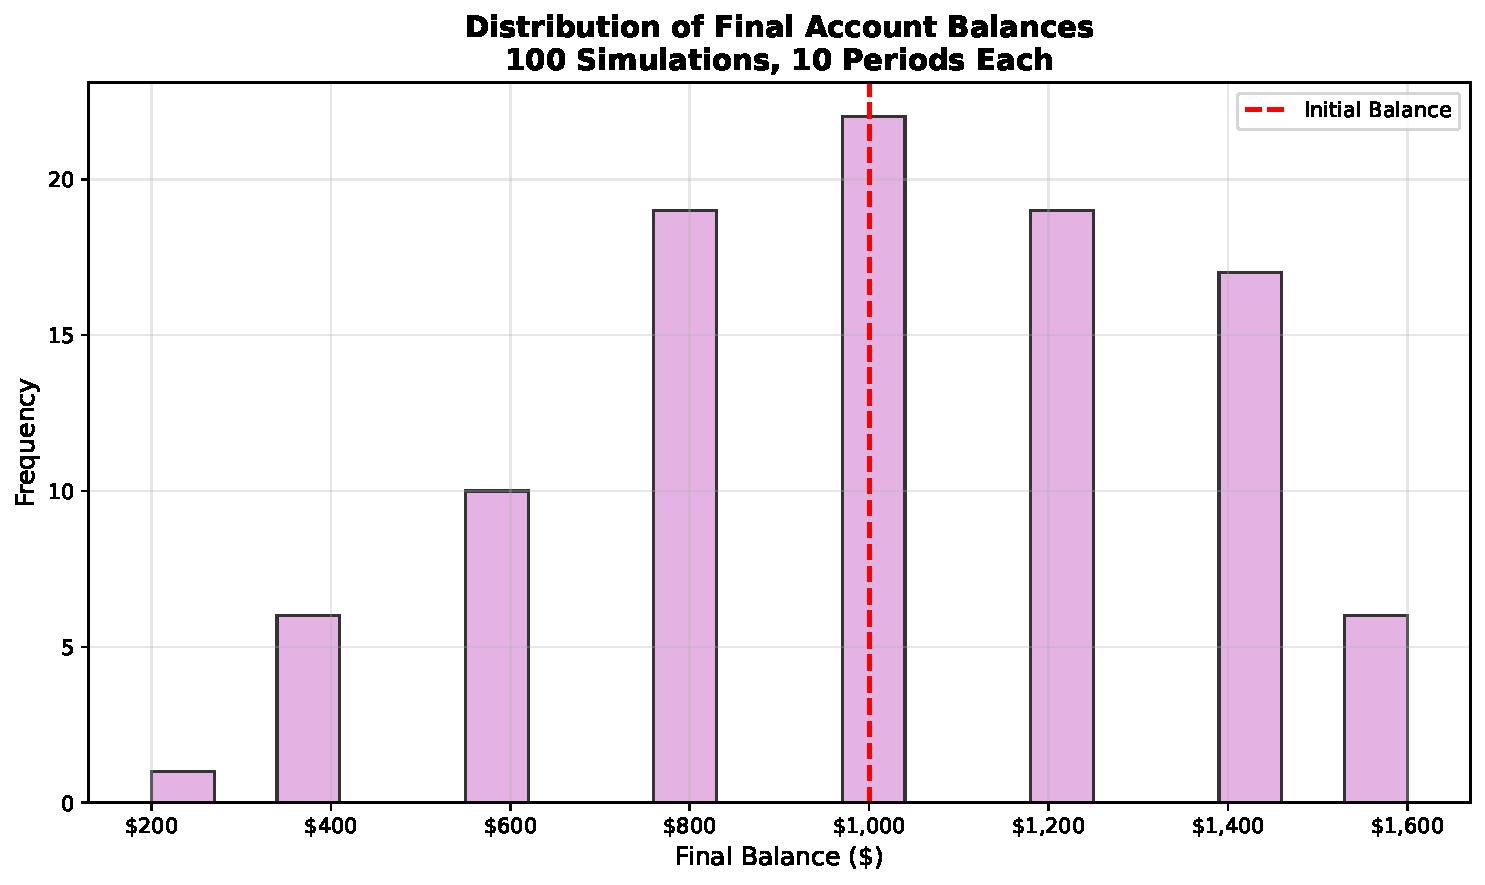
\includegraphics[keepaspectratio]{index_files/figure-pdf/distribution-sim-python-output-1.pdf}}

}

\caption{Python probability distribution of final balances}

\end{figure}%

\begin{verbatim}
Summary Statistics:
Mean balance: $1,020.00
Median balance: $1,000.00
Probability above initial: 0.420
\end{verbatim}




\end{document}
